\documentclass[UTF8]{ctexart}

%固定图片位置
\usepackage{float}

%插入超链接
\usepackage{url}

\usepackage{tikz,mathpazo}
\usetikzlibrary{shapes.geometric, arrows}
\usetikzlibrary{calc}

%\usepackage[affil-it]{authblk}

\usepackage{listings}
%插入代码的配置
\definecolor{CPPLight}  {HTML} {686868}
\definecolor{CPPSteel}  {HTML} {888888}
\definecolor{CPPDark}   {HTML} {262626}
\definecolor{CPPBlue}   {HTML} {4172A3}
\definecolor{CPPGreen}  {HTML} {487818}
\definecolor{CPPBrown}  {HTML} {A07040}
\definecolor{CPPRed}    {HTML} {AD4D3A}
\definecolor{CPPViolet} {HTML} {7040A0}
\definecolor{CPPGray}  {HTML} {B8B8B8}
\lstset{
	language=Matlab,                                     % 设置语言
    columns=fixed,    
    breaklines = true,   
    basicstyle=\small ,
    numbers=left,                                        % 在左侧显示行号
    %frame=none,                                          % 不显示背景边框
    backgroundcolor=\color[RGB]{245,245,244},            % 设定背景颜色
    keywordstyle=\color[RGB]{40,40,255}\bfseries,                 % 设定关键字颜色
    %commentstyle=\color{red!10!green!70}\textit,    % 设置代码注释的颜色
    numberstyle=\tiny\color{darkgray},           % 设定行号格式
    commentstyle=\it\color[RGB]{0,96,96},                % 设置代码注释的格式
    stringstyle=\rmfamily\slshape\color[RGB]{128,0,0},   % 设置字符串格式
    showstringspaces=false,                              % 不显示字符串中的空格                           
    %morekeywords={True,alignas,continute,friend,register,true,alignof,decltype,goto,
    %reinterpret_cast,try,asm,defult,if,return,typedef,auto,delete,inline,short,
    %typeid,bool,do,int,signed,typename,break,double,long,sizeof,union,case,
    %dynamic_cast,mutable,static,unsigned,catch,else,namespace,static_assert,using,
    %char,enum,new,static_cast,virtual,char16_t,char32_t,explict,noexcept,struct,
    %void,export,nullptr,switch,volatile,class,extern,operator,template,wchar_t,
    %const,false,private,this,while,constexpr,float,protected,thread_local,
    %const_cast,for,public,throw,std,rand},
    emph={access,and,break,class,continue,def,del,elif ,else,%
	except,exec,finally,for,from,global,if,import,in,i s,%
	lambda,not,or,pass,print,raise,return,try,while, imshow, subplot, figure,%
    log, fft2, fftshift, abs, size, rgb2gray, imread},
    emphstyle=\color{CPPViolet}\bfseries, 
    emph={[2]True, False, None, self},
	emphstyle=[2]\color{green},
	emph={[3]from, import, as},
	emphstyle=[3]\color{blue},
	upquote=true,
	morecomment=[s]{"""}{"""},
    morecomment=[s]{\%}{},
	%commentstyle=\color{orange}\slshape,
    commentstyle=\color{red!10!green!70}\textit,    % 设置代码注释的颜色
	emph={[4]1, 2, 3, 4, 5, 6, 7, 8, 9, 0},
	emphstyle=[4]\color{red},
	emph={[5]numpy, np, plt},
	emphstyle=[5]\color{red},
	literate=*{:}{{\textcolor{blue}:}}{1}%
	{=}{{\textcolor{blue}=}}{1}%
	{-}{{\textcolor{blue}-}}{1}%
	{+}{{\textcolor{blue}+}}{1}%
	{*}{{\textcolor{blue}*}}{1}%
	{!}{{\textcolor{blue}!}}{1}%
	{(}{{\textcolor{blue}(}}{1}%
	{)}{{\textcolor{blue})}}{1}%
	{[}{{\textcolor{blue}[}}{1}%
	{]}{{\textcolor{blue}]}}{1}%
	{<}{{\textcolor{blue}<}}{1}%
	{>}{{\textcolor{blue}>}}{1},%
    %{\%}{{\textcolor{green}\%}}{1},%
	framexleftmargin=0.1mm, framextopmargin=0.1mm, frame=shadowbox, rulesepcolor=\color{black},
}



\usepackage{geometry}
\geometry{left=1.2cm, right=1.2cm, top=1.2cm, bottom=1.2cm}

%得到引用的标题内容
\usepackage{nameref} 

%添加首行缩进,两个字符
\usepackage{indentfirst}
\setlength{\parindent}{2em}

%多行公式一个编号
\usepackage{amsmath}

%文献引用,标准类型为plain
%\usepackage[hyperref=true,backend=biber,sorting=none,backref=true]{biblatex}
%\addbibresource{ref.bib}
\bibliographystyle{plain}
\usepackage{cite}

\pagestyle{plain}

%跨页表格
\usepackage{multirow}
\usepackage{longtable,booktabs}
\usepackage{supertabular}
\usepackage{makecell}

%调整itemize等的间距
\usepackage{enumitem}


\usepackage{graphicx}
\usepackage{subfigure}

%超链接
\usepackage[linkcolor=yellow,citecolor=red,backref=page,hyperfootnotes=true]{hyperref}
\hypersetup{
bookmarks=true,
colorlinks=true,
linkcolor=black
}
\usepackage{tabularx} %This package must be placed after package {hyperref}, otherwise footnote marks are NOT treated as hyperlinks.


%引入了一些改进的数学环境,如align
\usepackage{amsmath}

\title{数字图像处理实验报告六}
\author{姓名:鲁国锐 \protect\newline
\and 学号:17020021031 \\
\and 专业:电子信息科学与技术}
%\date{2020年4月22日}

\begin{document}
	\maketitle
	\renewcommand{\contentsname}{目录}
	\renewcommand{\listfigurename}{插图目录}
	\renewcommand{\listtablename}{表格目录}
	\renewcommand{\refname}{参考文献}
	\renewcommand{\abstractname}{摘要}
	\renewcommand{\indexname}{索引}
	\renewcommand{\tablename}{表}
	\renewcommand{\figurename}{图}
	
	
	
	\tableofcontents
	\newpage
	
	\hypersetup{
	bookmarks=true,
	colorlinks=true,
	linkcolor=red,
	urlcolor=blue
	}
    
    \section{实验目标及要求}
        \indent 对$test$目录下的图像进行图像压缩测试,调节参数查看效果。  


    \section{实验}
        
        \subsection{基本思路}

                
            \indent 运行$Compressiontest.m$文件,修改其中$im2jpeg2k$函数的参数,观察结果变化。  
                
            \indent $Compressiontest$代码思路:读取一幅图像,将其转为灰度图,进行压缩,再解压缩,最后显示原图和恢复后的图像并计算压缩率。
                   
        
        \subsection{各函数功能说明}
        
            \subsubsection{$im2jpeg2k$函数}
                
                \indent 该函使用$jpeg2000$标准对图像进行编码压缩。
                
                \indent 该函数有三个输入量:
                \begin{enumerate}[leftmargin=50pt]
    				\item $X$:待压缩图像;
                    \item $N$:小波变换的尺度,该参数的值必须在$\left[ 1, \log_2\left(max\left(size\left( f \right)\right) \right) \right]$之间;
                    \item $Q$:量化步长,当提供两元素向量作为该参数时,使用隐式量化,如果输入向量长度不是$2$,函数将采用显式量化,并且必须提供大小为$3N_L+1$的步长(这里$N_L$是被计算的尺度数)。
    			\end{enumerate}
                
                \indent 本实验中,第三个参数均采用两元素向量。                
         
            \subsubsection{$jpeg2k2im$函数}
                
                \indent 该函数用于对被用$jpeg2000$标准编码的图像进行解码,输入只有一个参数,就是被编码的图像,输出即为解码后的图像。
         
            \subsubsection{$imratio$函数}
            
                \indent 该函数用于计算原图与压缩后的图像之间的压缩率。输入有两个参数,第一个为原图,第二个为编码后的图像。输出为压缩率。
                
            
        \subsection{代码实现}
           
             \begin{lstlisting}[language=Matlab,caption={$Compressiontest$代码},label={broadcast.cpp}]
 f=imread('test\euro2016.jpg'); % 读取图像
 f=rgb2gray(f); % 读取灰度图
 %存放路径
 path = 'C:\Users\Asus-\Desktop\数字图像\report\experience06\实验六 数学形态学及图像压缩\实验六 数学形态学及图像压缩\report\';
 imwrite(f, strcat(path, 'orig.jpg')); % 保存原图
 figure
 imshow(f) % 显示原图
 c1=im2jpeg2k(f,5,[8 8.5]); % 进行jpeg2000编码
 f1=jpeg2k2im(c1); % 解码
 figure
 imshow(f1); % 显示经过一次编解码之后的图像
 imwrite(f1, strcat(path, 'n_5_q_8_8-5.jpg')); % 保存结果
 imratio(f,c1) % 计算压缩率
 


              \end{lstlisting}
    

        \subsection{结果展示}
        
             			\begin{figure}[H]
             				\centering 
             				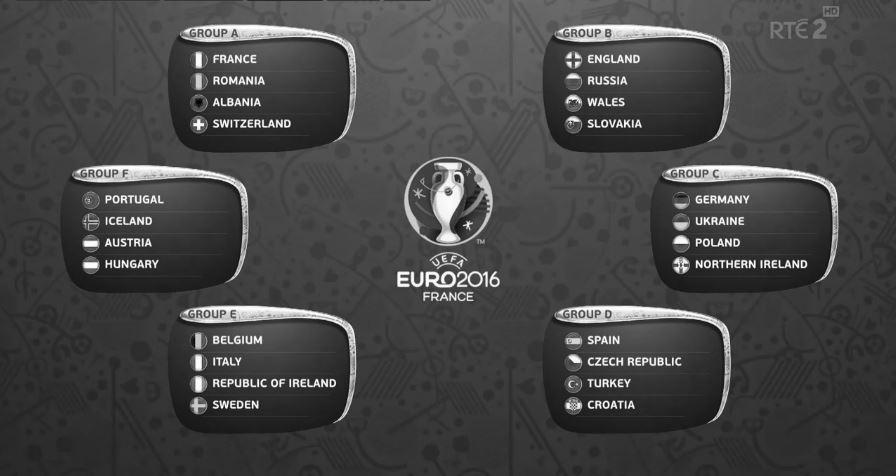
\includegraphics[scale=0.4]{orig.jpg} 
             				\caption{原图} 
             				\label{orig}
             			\end{figure}
                         
             			\begin{figure}[H]
             				\centering 
             				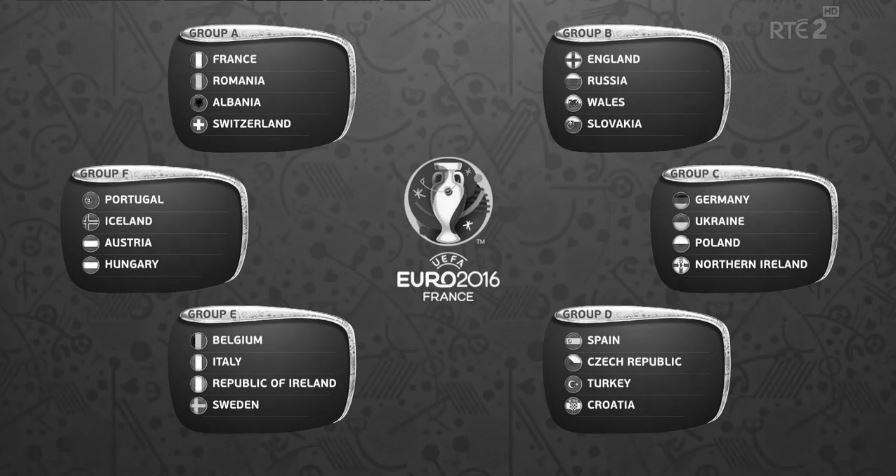
\includegraphics[scale=0.4]{n_1_q_8_8-5.jpg} 
             				\caption{$N = 1$,$Q = [8, 8.5]$时的结果,压缩率为$2.2833$} 
             				\label{n=1, Q=[8,8.5]}
             			\end{figure}                                          

             			\begin{figure}[H]
             				\centering 
             				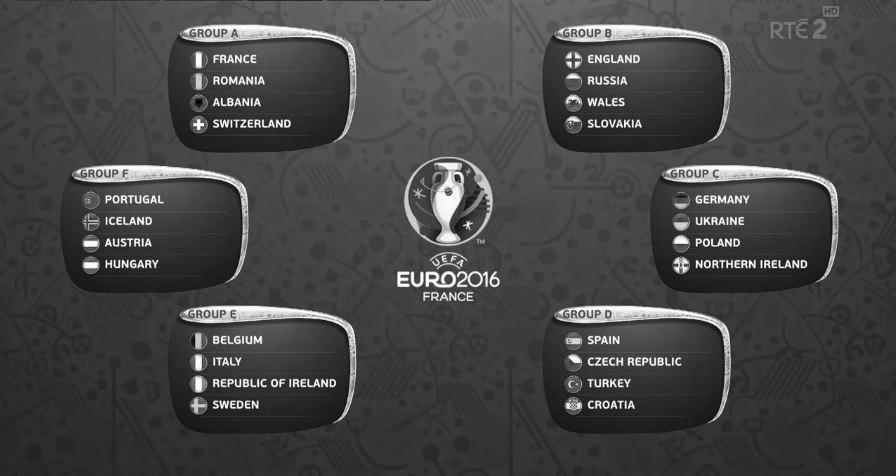
\includegraphics[scale=0.4]{n_2_q_8_8-5.jpg} 
             				\caption{$N = 2$,$Q = [8, 8.5]$时的结果,压缩率为$3.9933$} 
             				\label{n=2, Q=[8,8.5]}
             			\end{figure}
                         
             			\begin{figure}[H]
             				\centering 
             				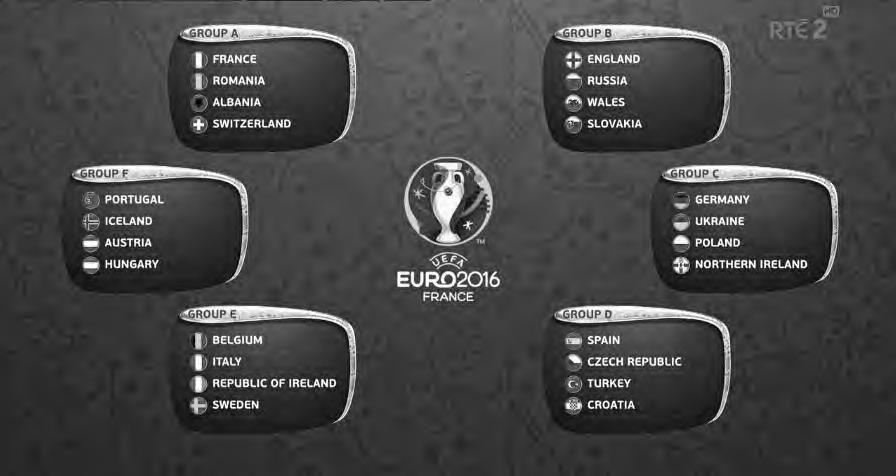
\includegraphics[scale=0.4]{n_5_q_8_8-5.jpg} 
             				\caption{$N = 5$,$Q = [8, 8.5]$时的结果,压缩率为$15.4382$} 
             				\label{n=5, Q=[8,8.5]}
             			\end{figure} 
                         
             			\begin{figure}[H]
             				\centering 
             				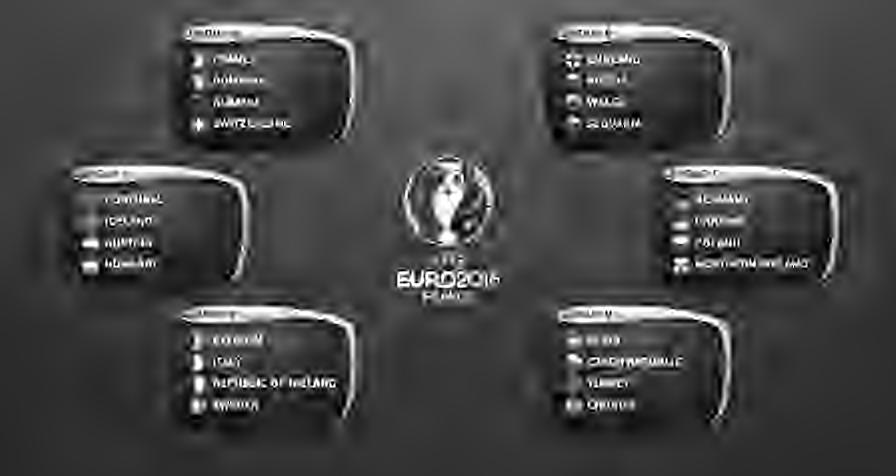
\includegraphics[scale=0.4]{n_8_q_8_8-5.jpg} 
             				\caption{$N = 8$,$Q = [8, 8.5]$时的结果,压缩率为$114.1585$} 
             				\label{n=8, Q=[8,8.5]}
             			\end{figure} 
                         
             			\begin{figure}[H]
             				\centering 
             				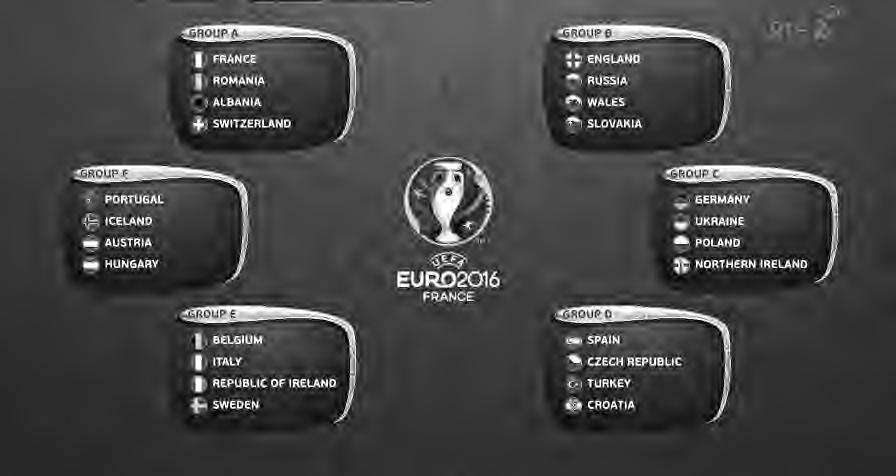
\includegraphics[scale=0.4]{n_5_q_8_7.jpg} 
             				\caption{$N = 5$,$Q = [8, 7]$时的结果,压缩率为$33.2576$} 
             				\label{n=5, Q=[8,7]}
             			\end{figure}
                         
             			\begin{figure}[H]
             				\centering 
             				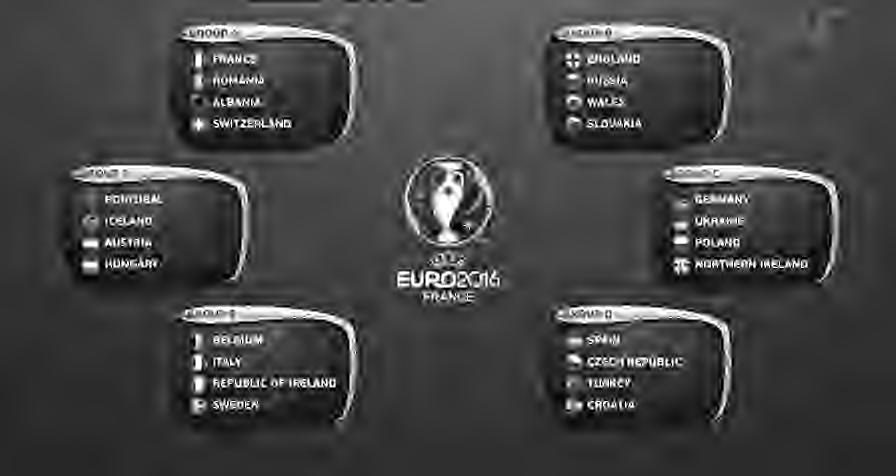
\includegraphics[scale=0.4]{n_5_q_8_6.jpg} 
             				\caption{$N = 5$,$Q = [8, 6]$时的结果,压缩率为$69.3039$} 
             				\label{n=5, Q=[8,6]}
             			\end{figure} 
                         
             			\begin{figure}[H]
             				\centering 
             				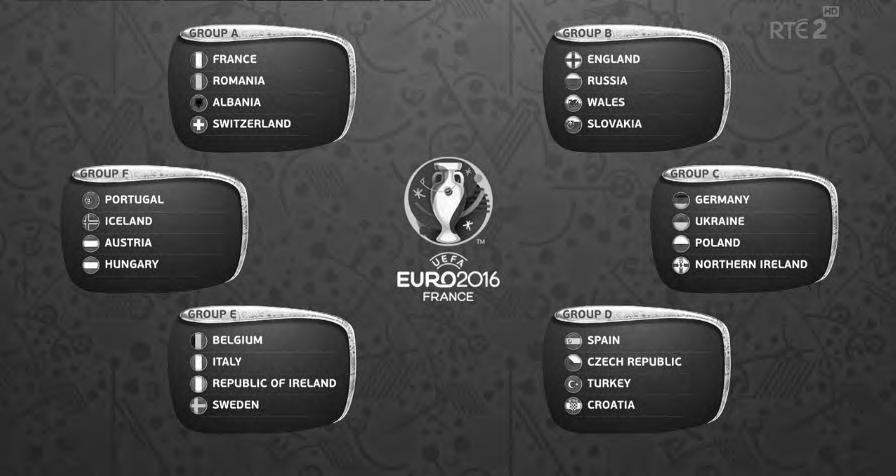
\includegraphics[scale=0.4]{n_5_q_8_10.jpg} 
             				\caption{$N = 5$,$Q = [8, 10]$时的结果,压缩率为$8.0271$} 
             				\label{n=5, Q=[8,10]}
             			\end{figure}                                                                                                        
                         
             			\begin{figure}[H]
             				\centering 
             				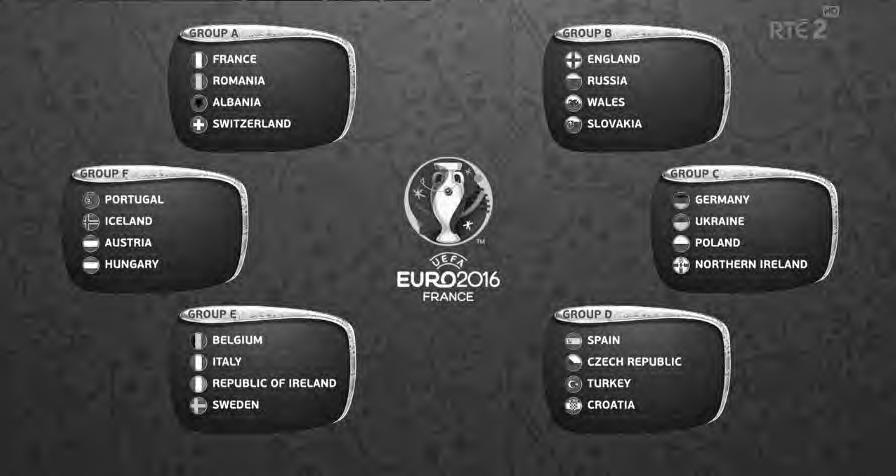
\includegraphics[scale=0.4]{n_5_q_7_8-5.jpg} 
             				\caption{$N = 5$,$Q = [7, 8.5]$时的结果,压缩率为$15.4282$} 
             				\label{n=5, Q=[7,8.5]}
             			\end{figure}  
                         
             			\begin{figure}[H]
             				\centering 
             				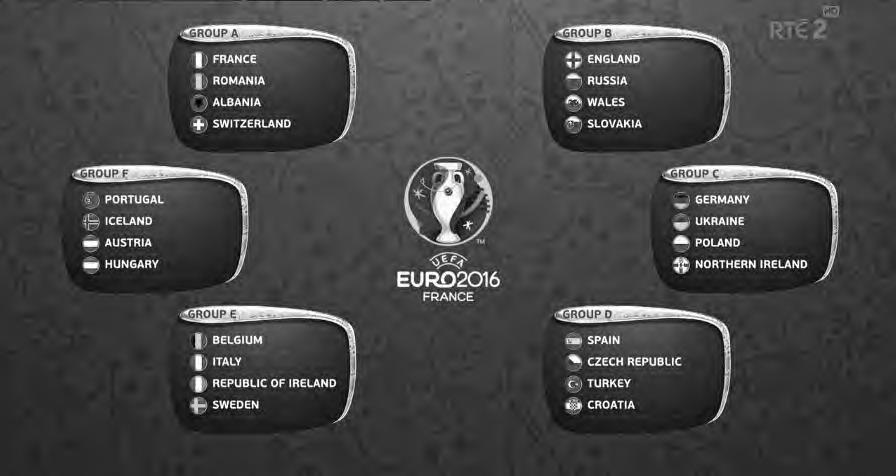
\includegraphics[scale=0.4]{n_5_q_6_8-5.jpg} 
             				\caption{$N = 5$,$Q = [6, 8.5]$时的结果,压缩率为$15.4237$} 
             				\label{n=5, Q=[6,8.5]}
             			\end{figure} 
                         
             			\begin{figure}[H]
             				\centering 
             				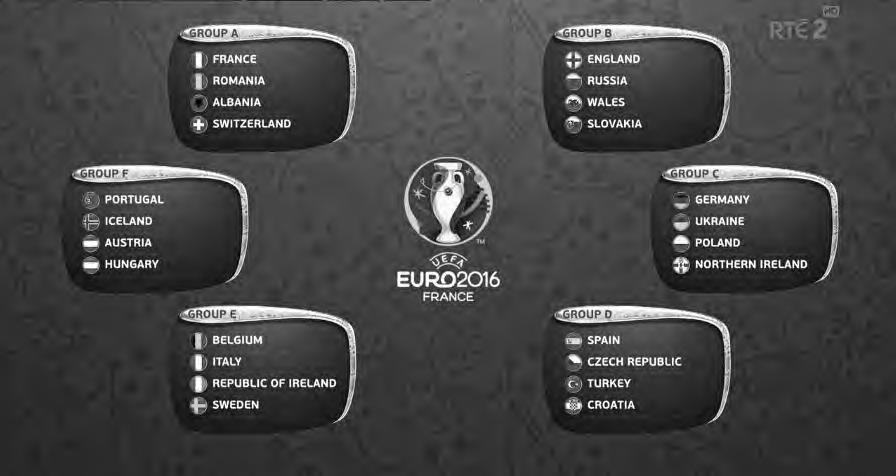
\includegraphics[scale=0.4]{n_5_q_10_8-5.jpg} 
             				\caption{$N = 5$,$Q = [10, 8.5]$时的结果,压缩率为$15.4449$} 
             				\label{n=5, Q=[10,8.5]}
             			\end{figure}                                                                                   
                        
%                        \begin{figure}[H]
%                            \centering
%                            \subfigure[原图的灰度图]{
%                                \begin{minipage}{0.45\linewidth}
%                                    \centering
%                                    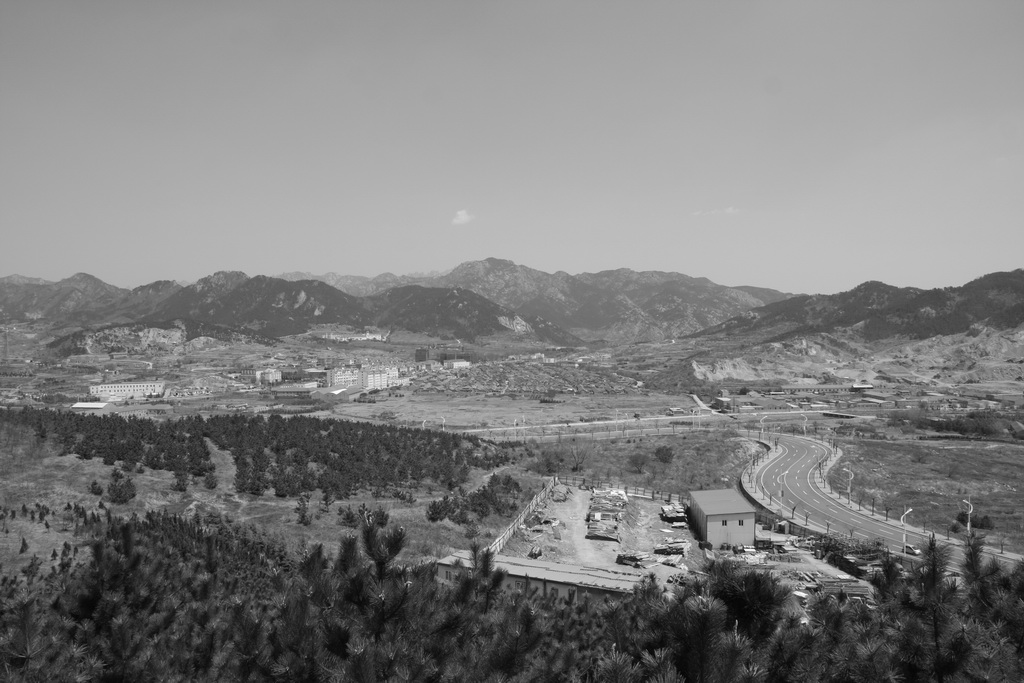
\includegraphics[scale=0.2]{n_eq_4_orig.png}
%                                    %\caption{原图3}
%                                \end{minipage}
%                            }
%                            \subfigure[小波变换结果]{
%                                \begin{minipage}{0.45\linewidth}
%                                    \centering
%                                    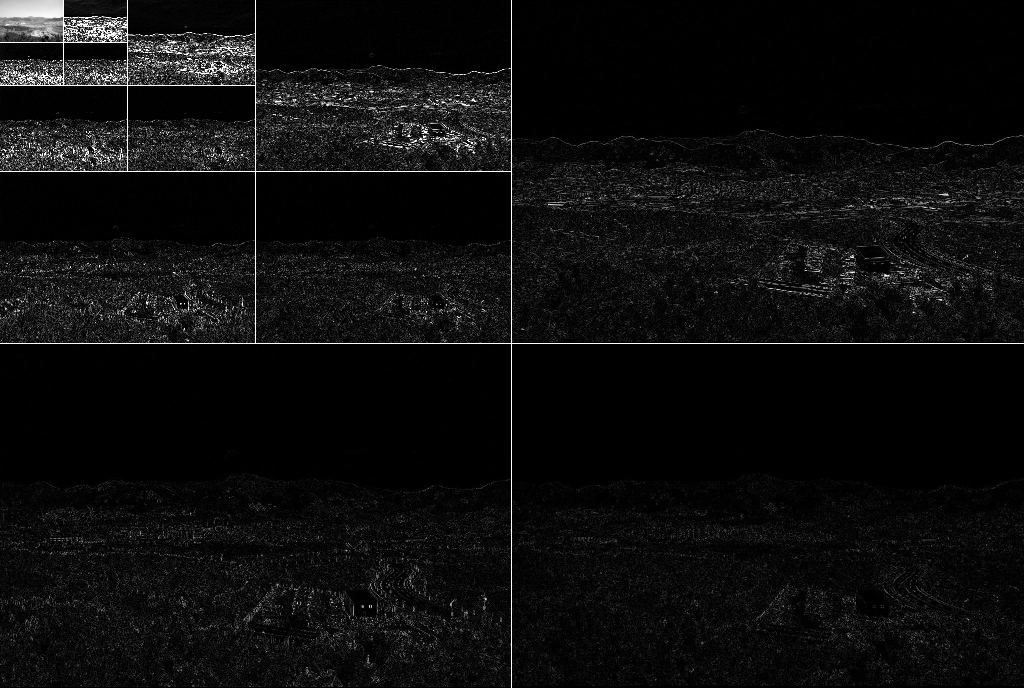
\includegraphics[scale=0.2]{n_eq_4_FWT.png}
%                                    %\caption{结果3}
%                                    \label{n_eq_4_FWT}
%                                \end{minipage}
%                            }
%                            \subfigure[消除近似分量后的变换结果]{
%                                \begin{minipage}{0.45\linewidth}
%                                    \centering
%                                    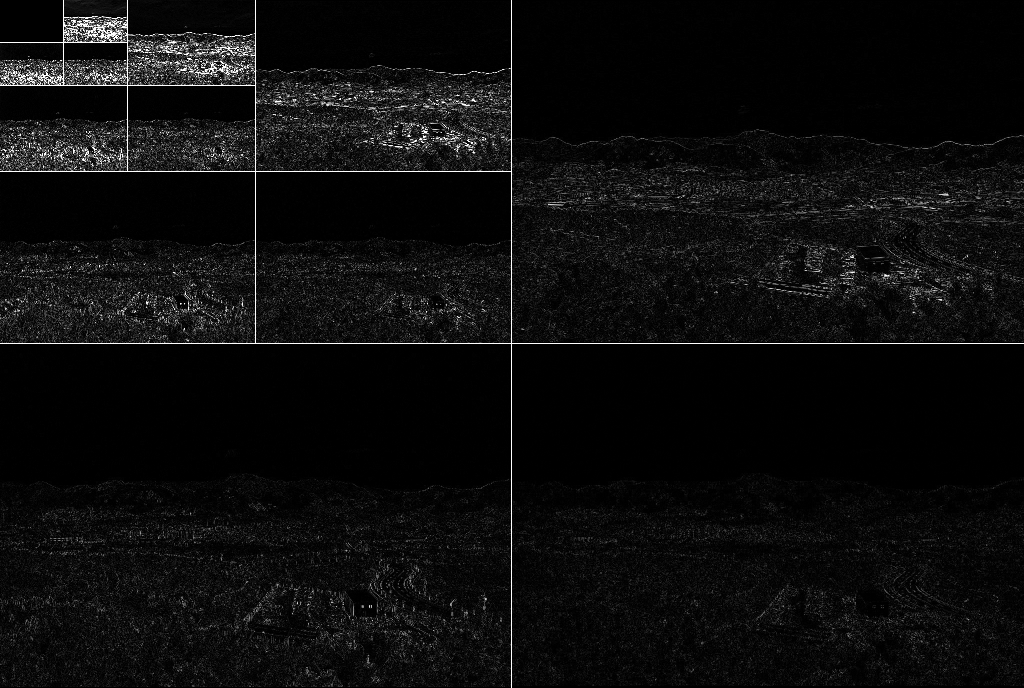
\includegraphics[scale=0.2]{n_eq_4_cut.png}
%                                    %\caption{结果3}
%                                    \label{n_eq_4_cut}
%                                \end{minipage}
%                            }  
%                            \subfigure[反变换后的结果:边缘增强]{
%                                \begin{minipage}{0.45\linewidth}
%                                    \centering
%                                    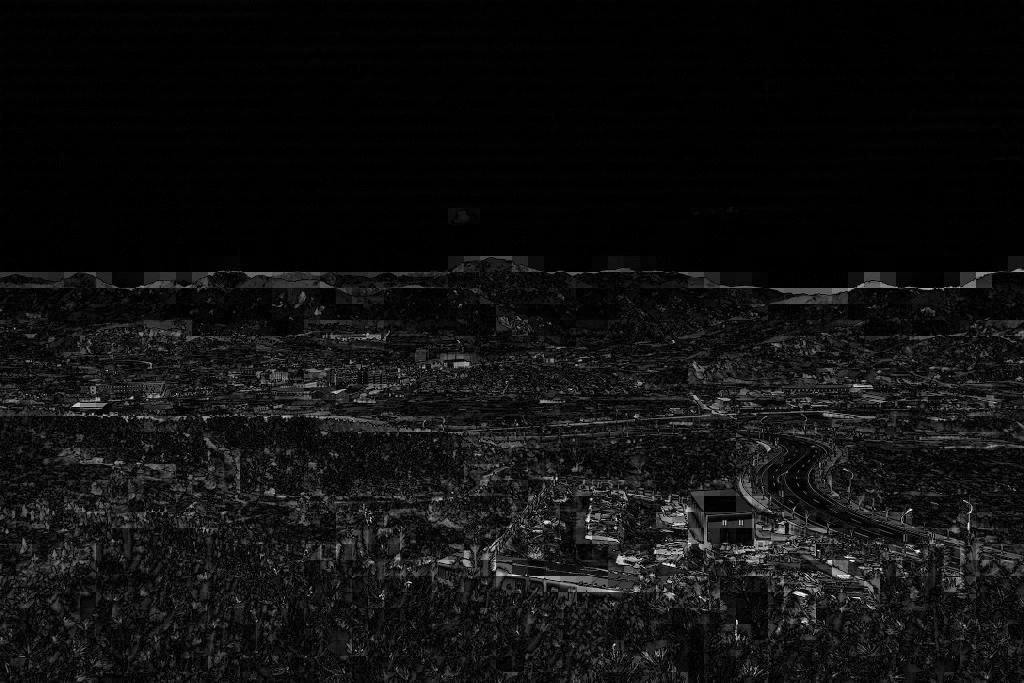
\includegraphics[scale=0.2]{n_eq_4_edge.png}
%                                    %\caption{结果3}
%                                    \label{n_eq_4_edge}
%                                \end{minipage}
%                            }                                                      
%                            
%                            \caption{$n$等于$4$时的实验结果}
%                            \label{n_eq_4}
%                        \end{figure}
%                        
%                        
%                        \begin{figure}[H]
%                            \centering
%                            \subfigure[原图的灰度图]{
%                                \begin{minipage}{0.45\linewidth}
%                                    \centering
%                                    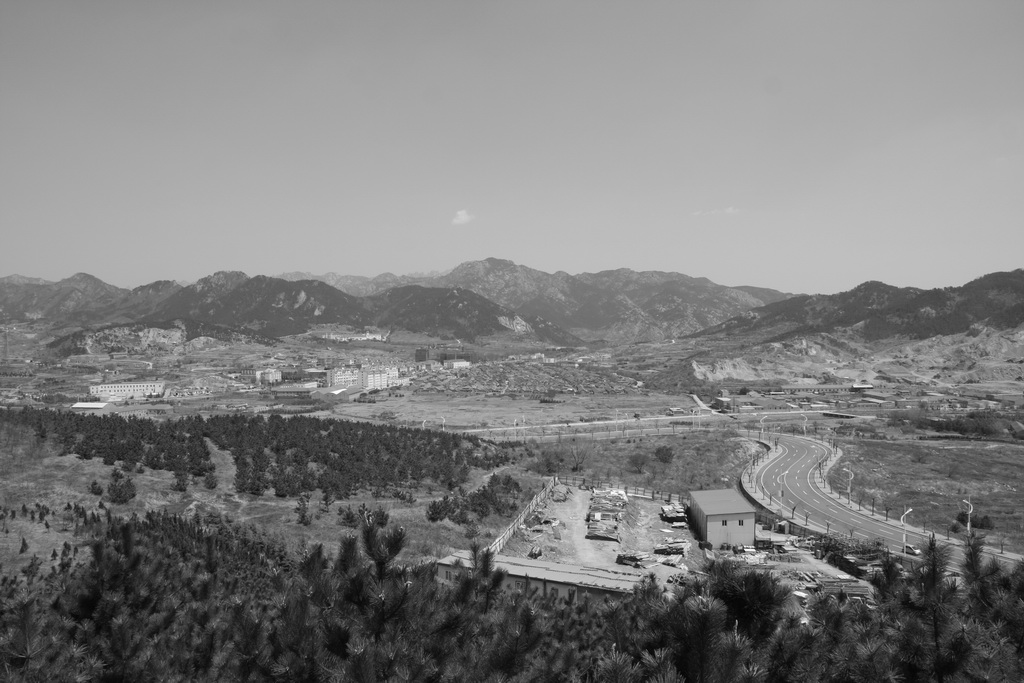
\includegraphics[scale=0.2]{n_eq_1_orig.png}
%                                    %\caption{原图3}
%                                \end{minipage}
%                            }
%                            \subfigure[小波变换结果]{
%                                \begin{minipage}{0.45\linewidth}
%                                    \centering
%                                    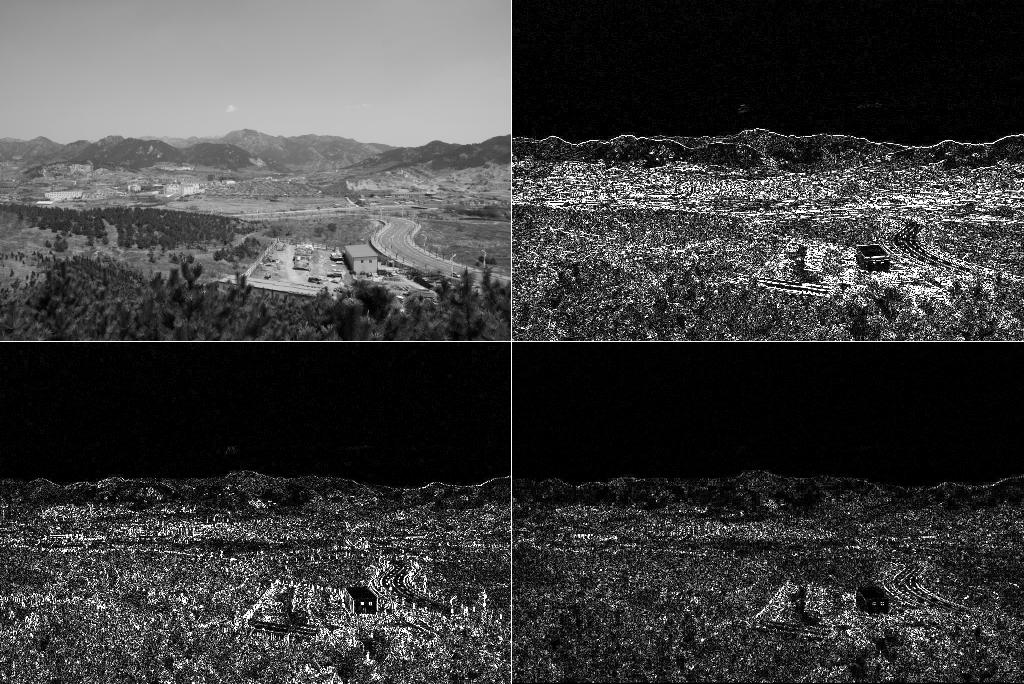
\includegraphics[scale=0.2]{n_eq_1_FWT.png}
%                                    %\caption{结果3}
%                                    \label{n_eq_1_FWT}
%                                \end{minipage}
%                            }
%                            \subfigure[消除近似分量后的变换结果]{
%                                \begin{minipage}{0.45\linewidth}
%                                    \centering
%                                    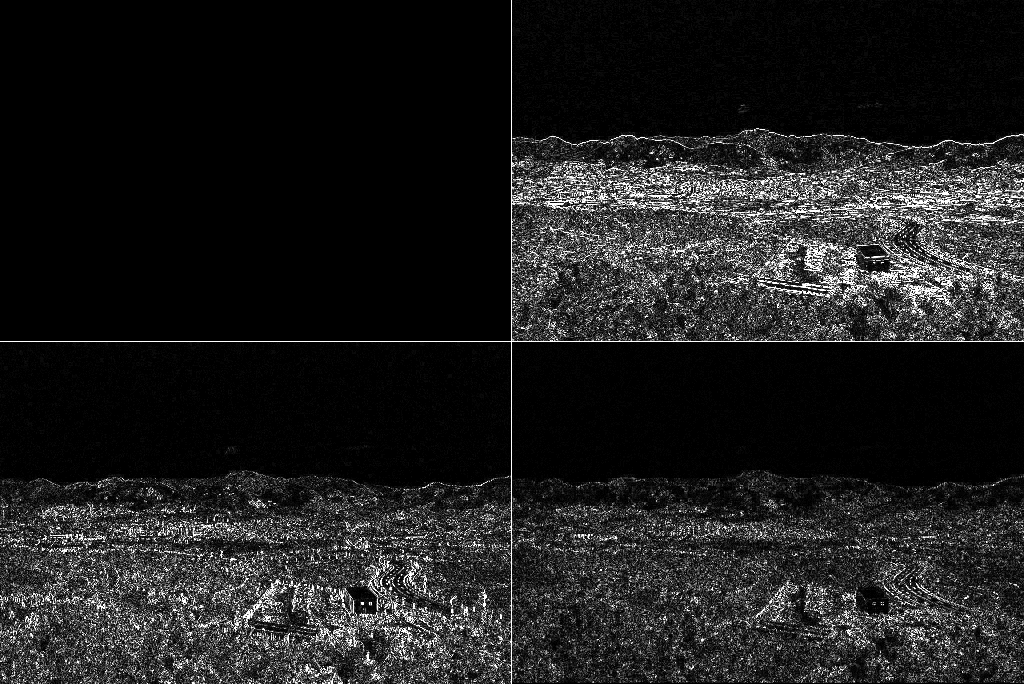
\includegraphics[scale=0.2]{n_eq_1_cut.png}
%                                    %\caption{结果3}
%                                    \label{n_eq_1_cut}
%                                \end{minipage}
%                            }  
%                            \subfigure[反变换后的结果:边缘增强]{
%                                \begin{minipage}{0.45\linewidth}
%                                    \centering
%                                    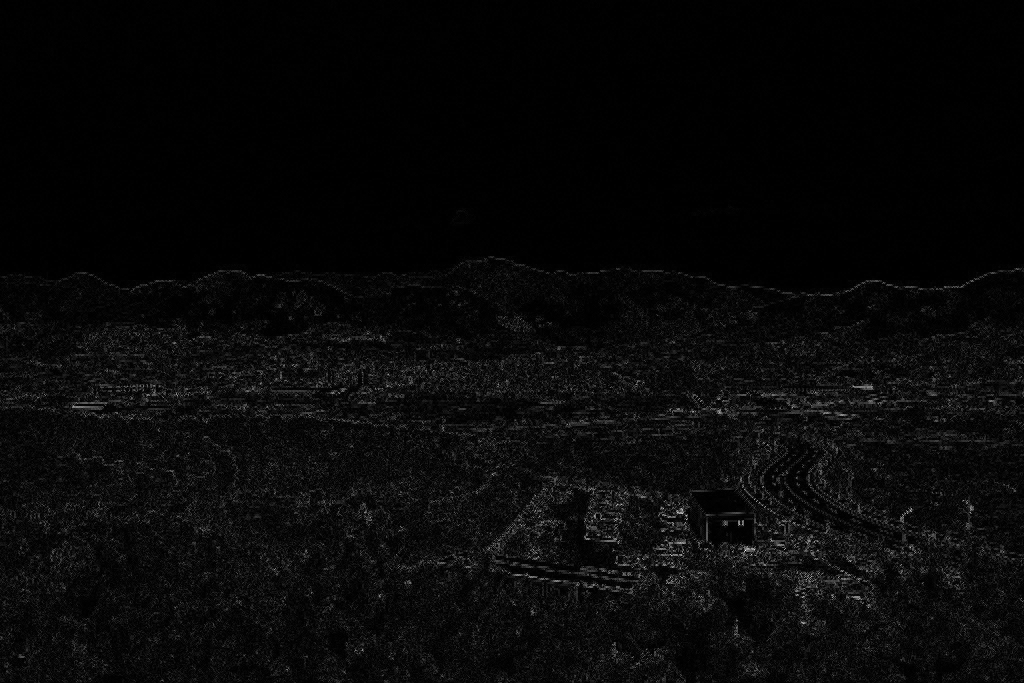
\includegraphics[scale=0.2]{n_eq_1_edge.png}
%                                    %\caption{结果3}
%                                    \label{n_eq_1_edge}
%                                \end{minipage}
%                            }                                                      
%                            
%                            \caption{$n$等于$1$时的实验结果}
%                            \label{n_eq_1}
%                        \end{figure} 
%                                               
%                        \begin{figure}[H]
%                            \centering
%                            \subfigure[原图的灰度图]{
%                                \begin{minipage}{0.45\linewidth}
%                                    \centering
%                                    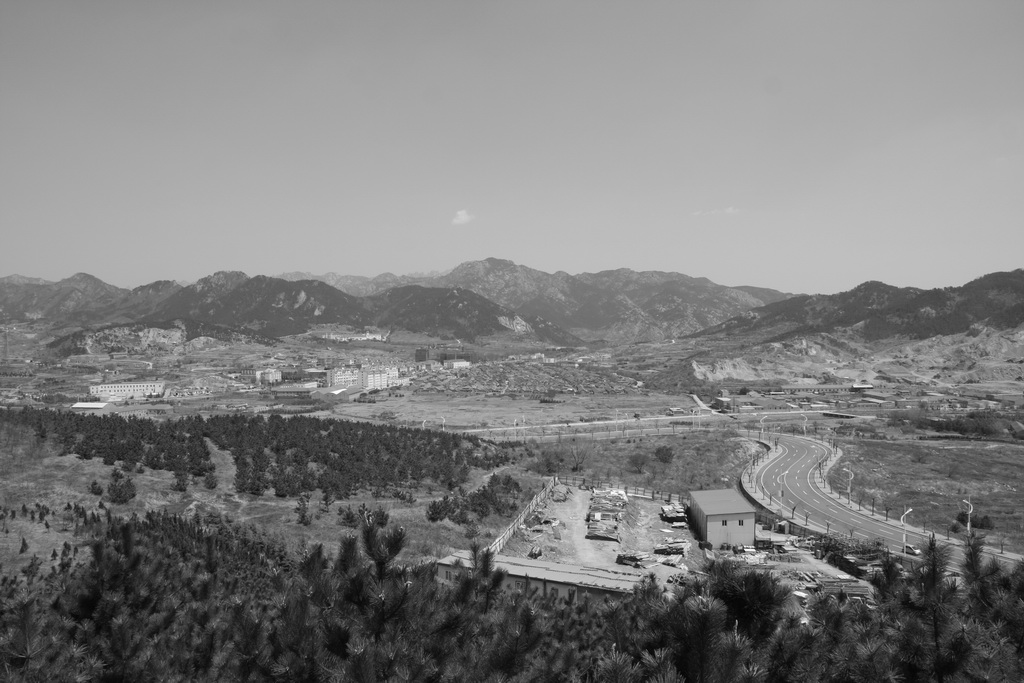
\includegraphics[scale=0.2]{n_eq_2_orig.png}
%                                    %\caption{原图3}
%                                \end{minipage}
%                            }
%                            \subfigure[小波变换结果]{
%                                \begin{minipage}{0.45\linewidth}
%                                    \centering
%                                    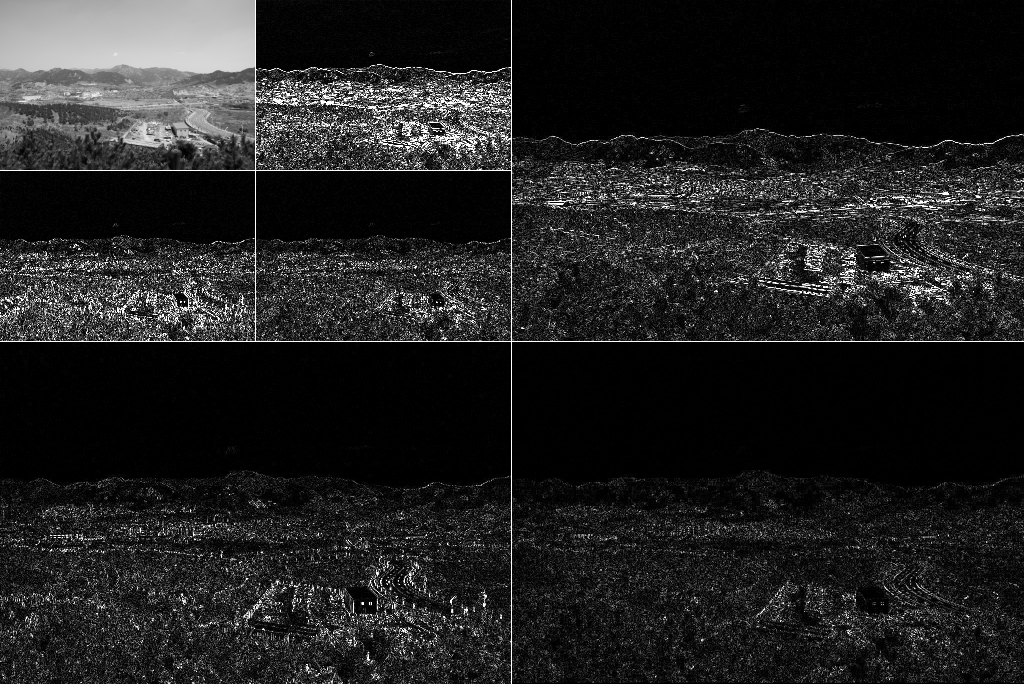
\includegraphics[scale=0.2]{n_eq_2_FWT.png}
%                                    %\caption{结果3}
%                                    \label{n_eq_2_FWT}
%                                \end{minipage}
%                            }
%                            \subfigure[消除近似分量后的变换结果]{
%                                \begin{minipage}{0.45\linewidth}
%                                    \centering
%                                    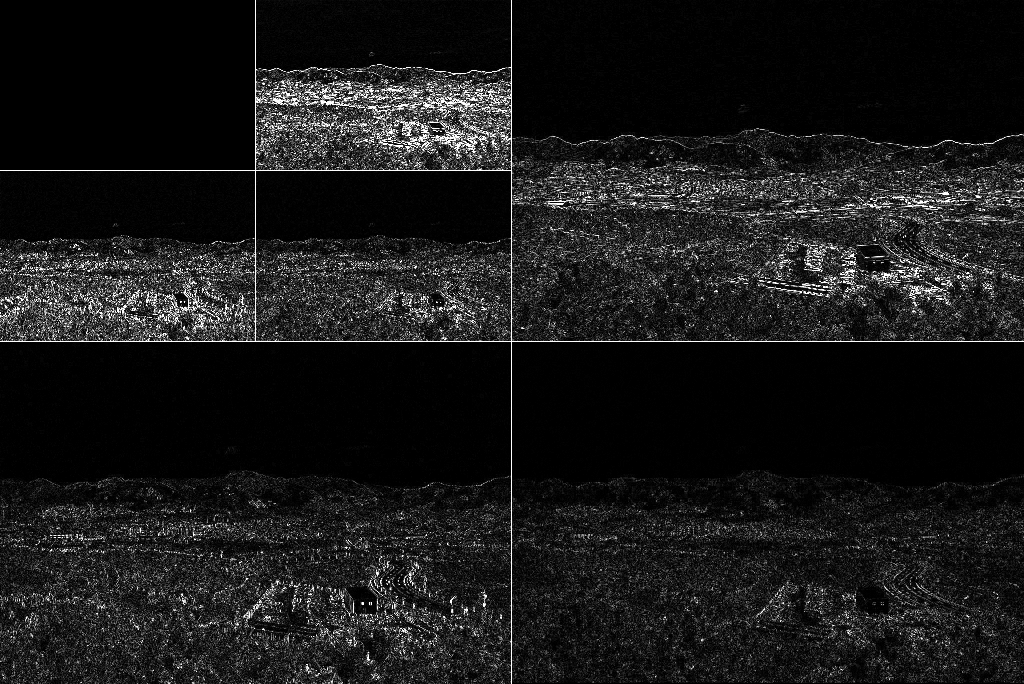
\includegraphics[scale=0.2]{n_eq_2_cut.png}
%                                    %\caption{结果3}
%                                    \label{n_eq_2_cut}
%                                \end{minipage}
%                            }  
%                            \subfigure[反变换后的结果:边缘增强]{
%                                \begin{minipage}{0.45\linewidth}
%                                    \centering
%                                    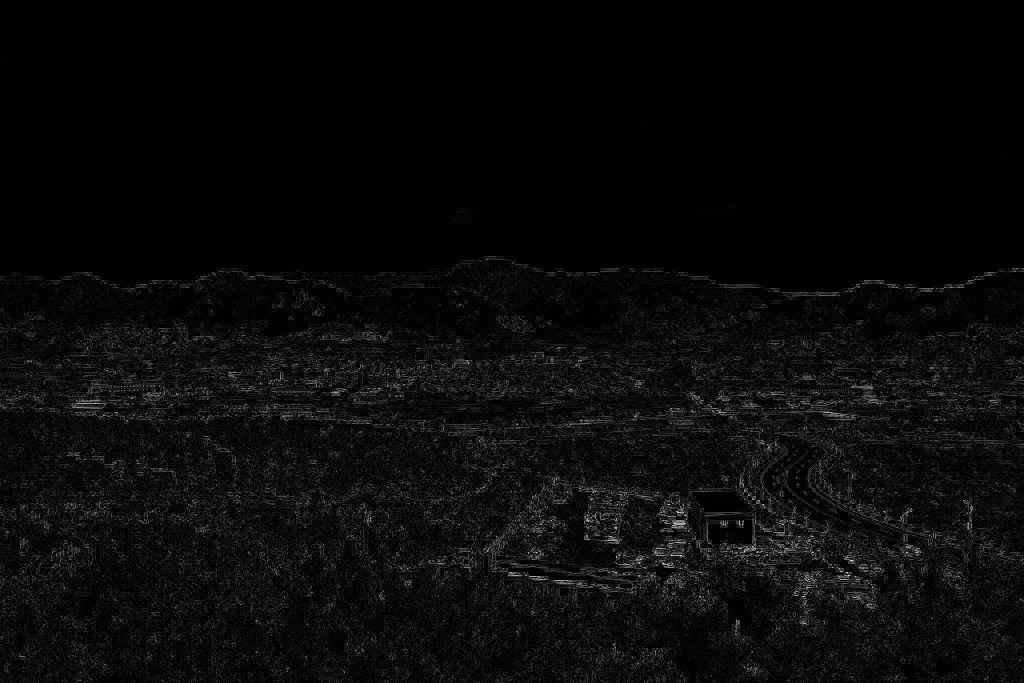
\includegraphics[scale=0.2]{n_eq_2_edge.png}
%                                    %\caption{结果3}
%                                    \label{n_eq_2_edge}
%                                \end{minipage}
%                            }                                                      
%                            
%                            \caption{$n$等于$2$时的实验结果}
%                            \label{n_eq_2}
%                        \end{figure}
%
%                        \begin{figure}[H]
%                            \centering
%                            \subfigure[原图的灰度图]{
%                                \begin{minipage}{0.45\linewidth}
%                                    \centering
%                                    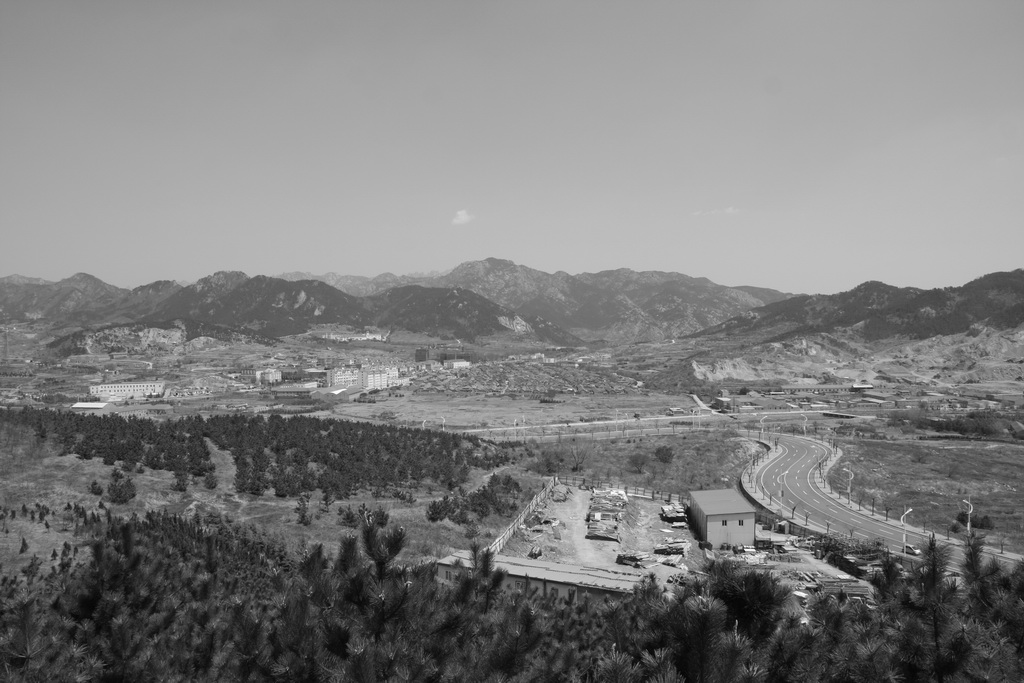
\includegraphics[scale=0.2]{n_eq_8_orig.png}
%                                    %\caption{原图3}
%                                \end{minipage}
%                            }
%                            \subfigure[小波变换结果]{
%                                \begin{minipage}{0.45\linewidth}
%                                    \centering
%                                    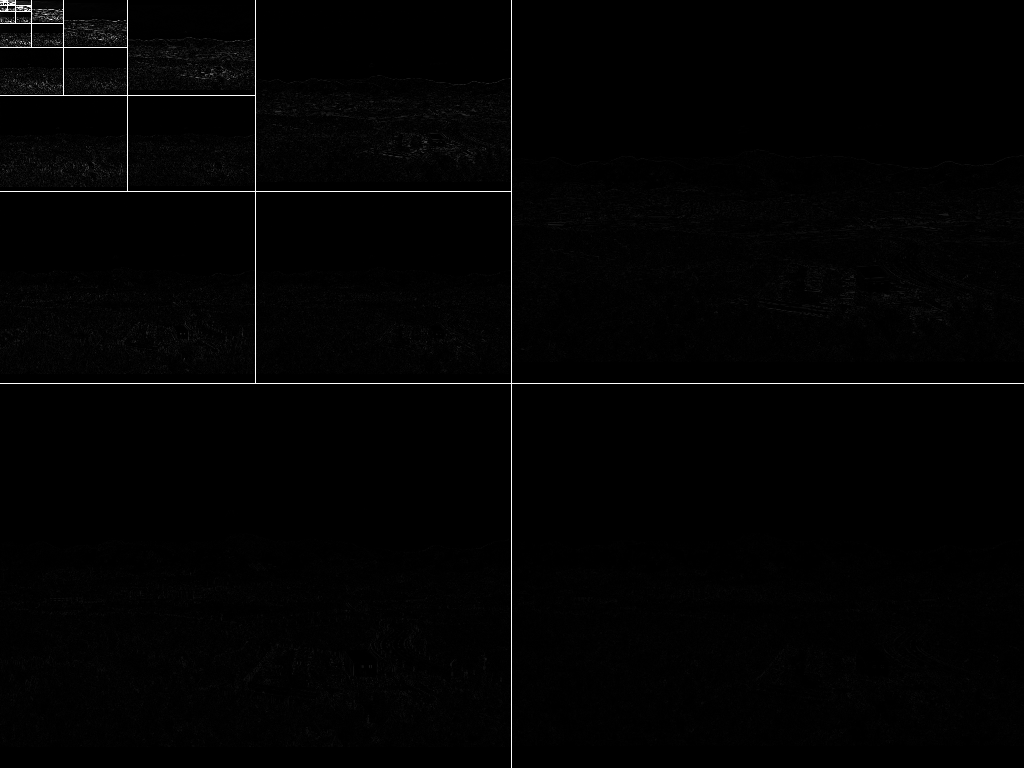
\includegraphics[scale=0.2]{n_eq_8_FWT.png}
%                                    %\caption{结果3}
%                                    \label{n_eq_8_FWT}
%                                \end{minipage}
%                            }
%                            \subfigure[消除近似分量后的变换结果]{
%                                \begin{minipage}{0.45\linewidth}
%                                    \centering
%                                    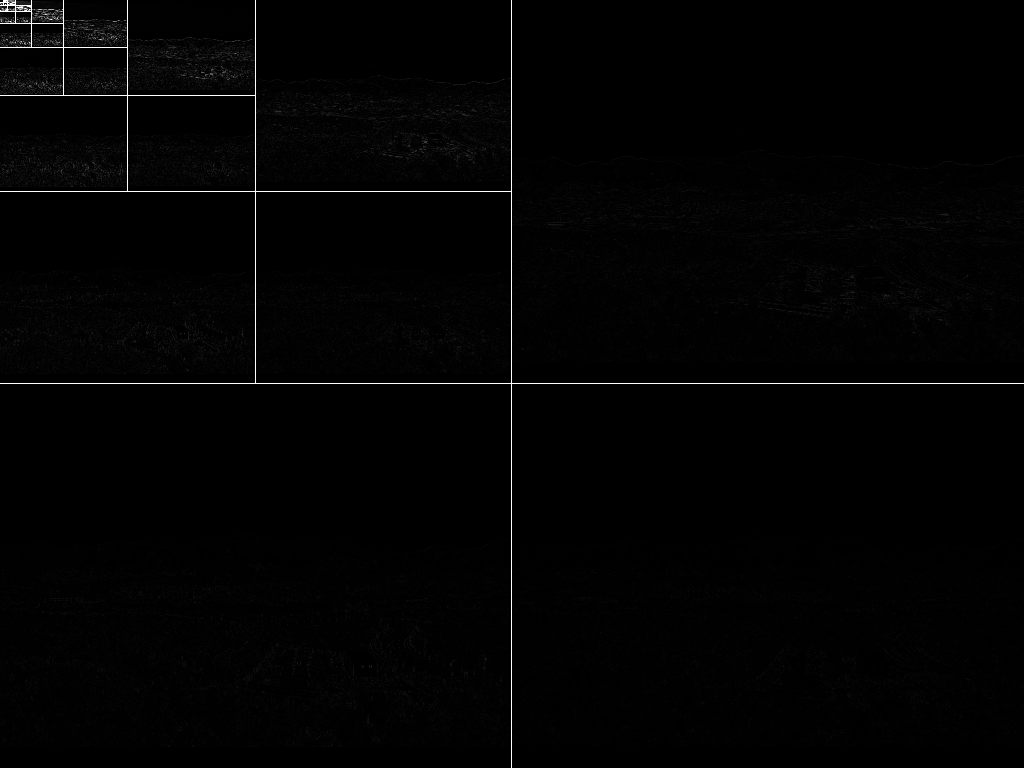
\includegraphics[scale=0.2]{n_eq_8_cut.png}
%                                    %\caption{结果3}
%                                    \label{n_eq_8_cut}
%                                \end{minipage}
%                            }  
%                            \subfigure[反变换后的结果:边缘增强]{
%                                \begin{minipage}{0.45\linewidth}
%                                    \centering
%                                    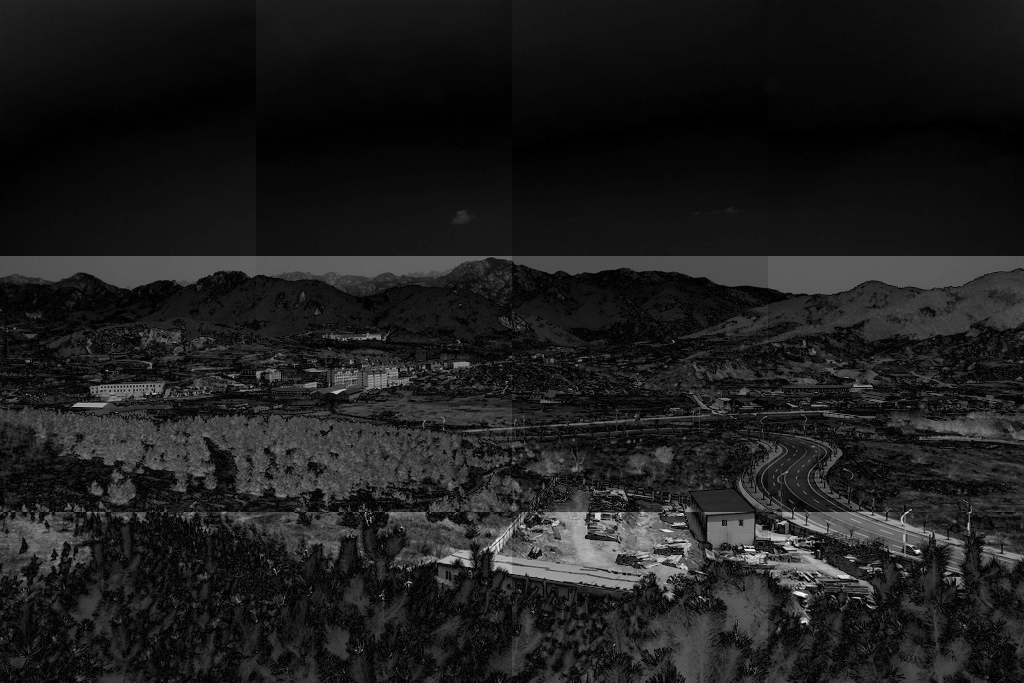
\includegraphics[scale=0.2]{n_eq_8_edge.png}
%                                    %\caption{结果3}
%                                    \label{n_eq_8_edge}
%                                \end{minipage}
%                            }                                                      
%                            
%                            \caption{$n$等于$8$时的实验结果}
%                            \label{n_eq_8}
%                        \end{figure}
%
%                        \begin{figure}[H]
%                            \centering
%                            \subfigure[原图的灰度图]{
%                                \begin{minipage}{0.45\linewidth}
%                                    \centering
%                                    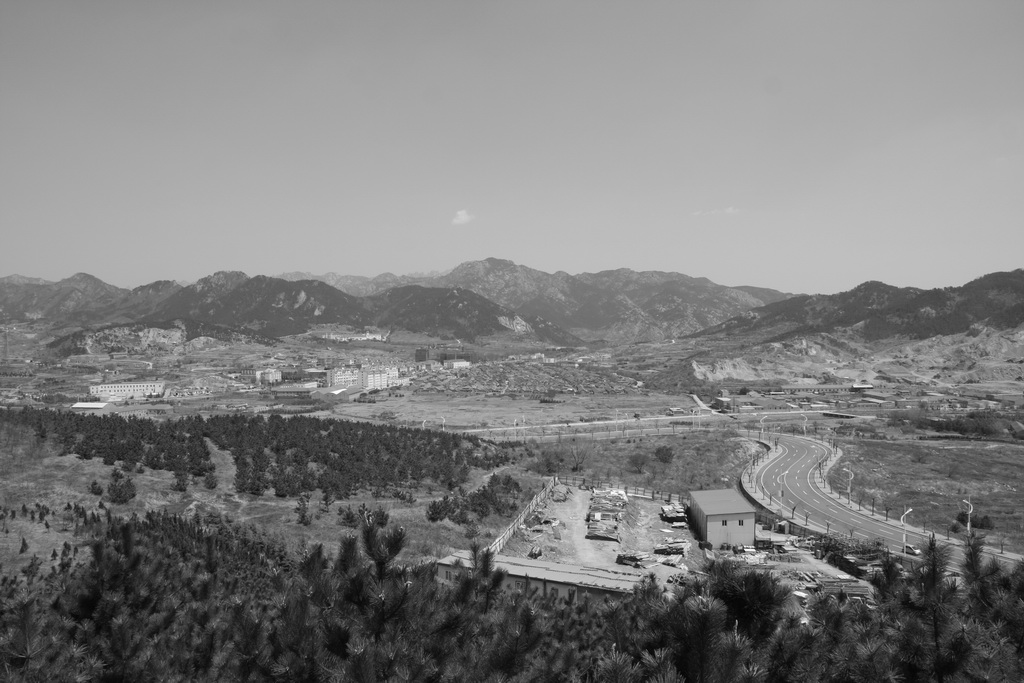
\includegraphics[scale=0.2]{n_eq_10_orig.png}
%                                    %\caption{原图3}
%                                \end{minipage}
%                            }
%                            \subfigure[小波变换结果]{
%                                \begin{minipage}{0.45\linewidth}
%                                    \centering
%                                    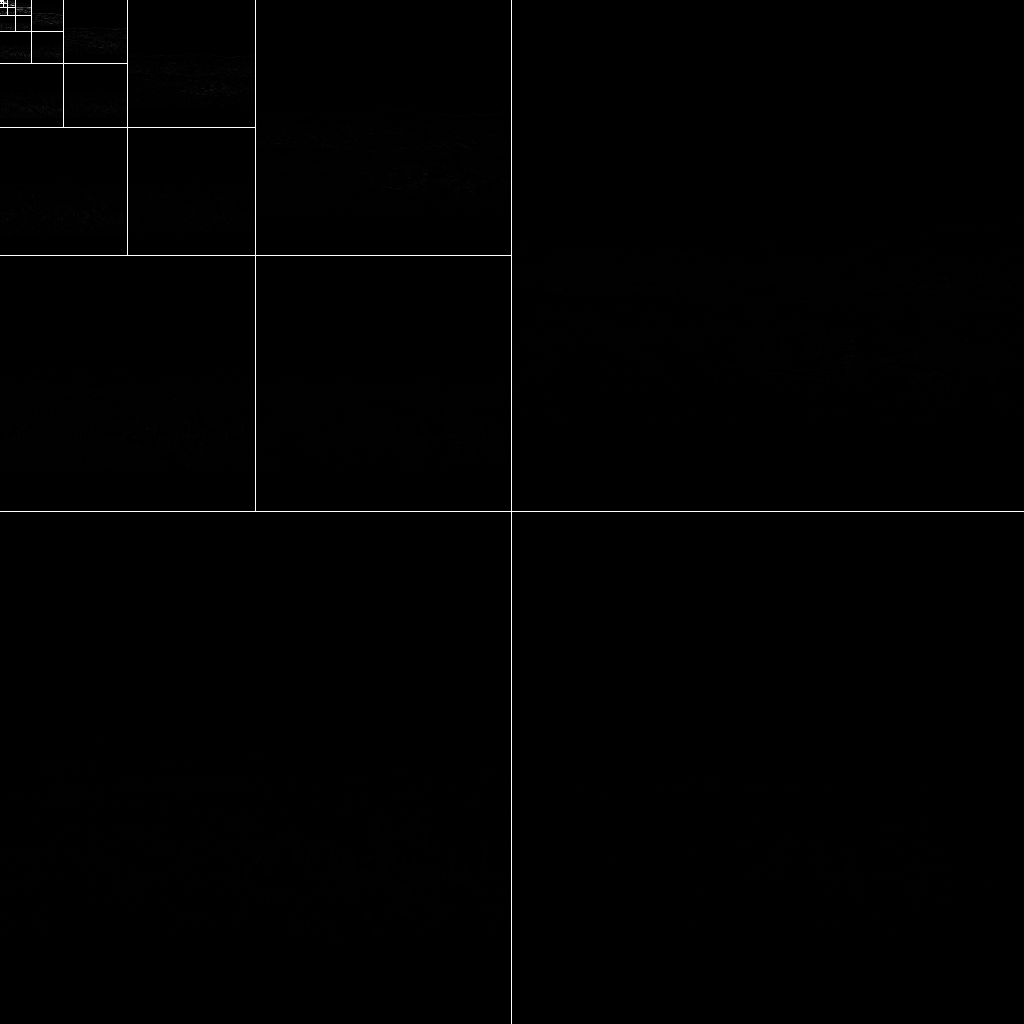
\includegraphics[scale=0.2]{n_eq_10_FWT.png}
%                                    %\caption{结果3}
%                                    \label{n_eq_10_FWT}
%                                \end{minipage}
%                            }
%                            \subfigure[消除近似分量后的变换结果]{
%                                \begin{minipage}{0.45\linewidth}
%                                    \centering
%                                    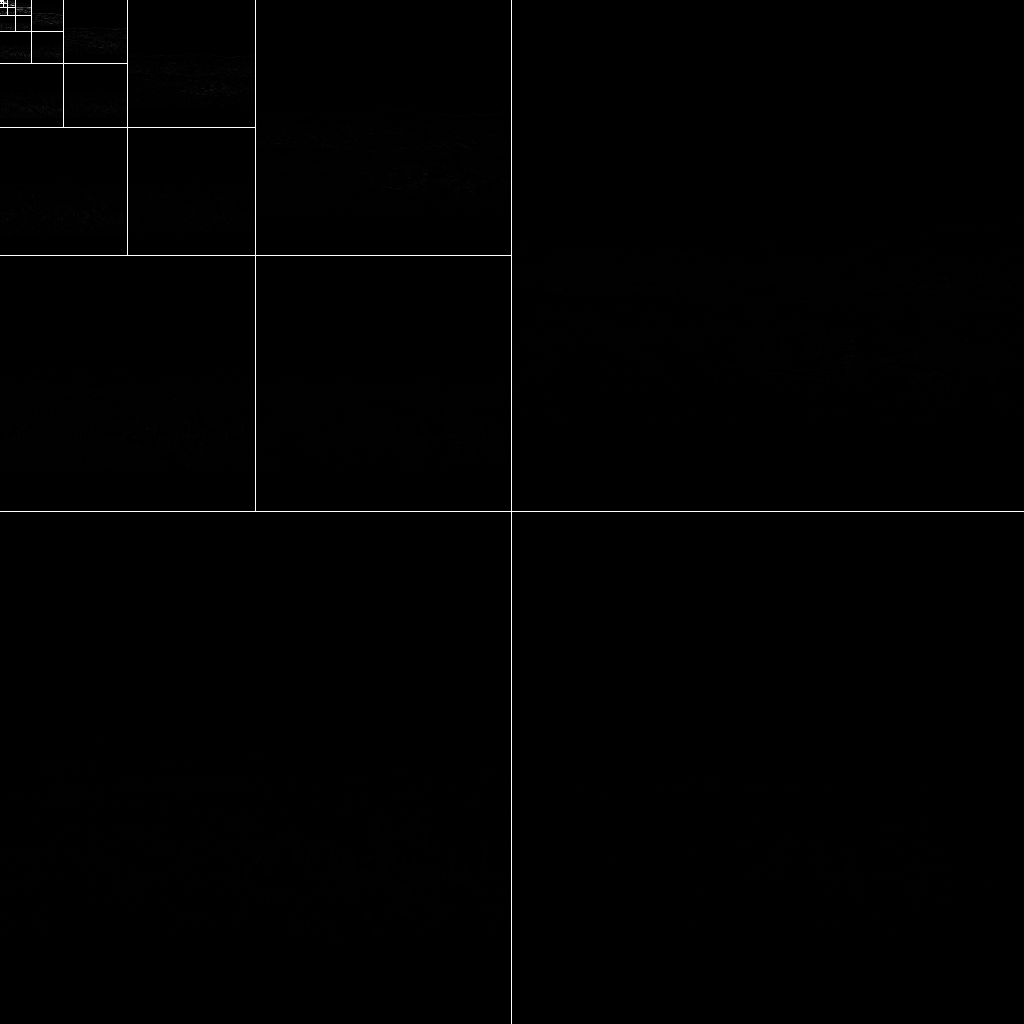
\includegraphics[scale=0.2]{n_eq_10_cut.png}
%                                    %\caption{结果3}
%                                    \label{n_eq_10_cut}
%                                \end{minipage}
%                            }  
%                            \subfigure[反变换后的结果:边缘增强]{
%                                \begin{minipage}{0.45\linewidth}
%                                    \centering
%                                    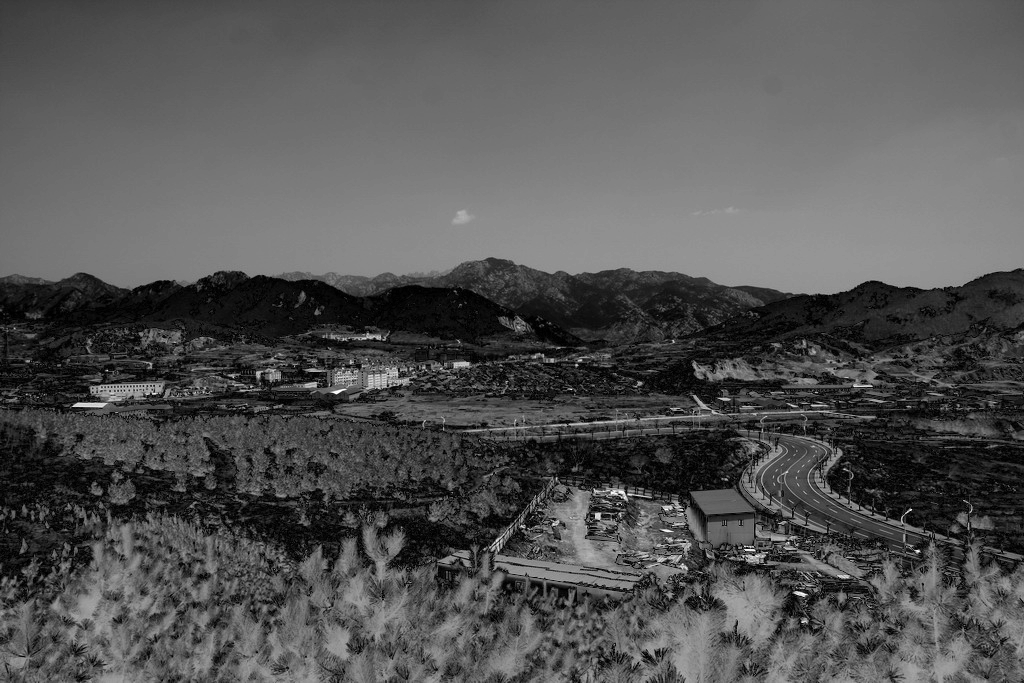
\includegraphics[scale=0.2]{n_eq_10_edge.png}
%                                    %\caption{结果3}
%                                    \label{n_eq_10_edge}
%                                \end{minipage}
%                            }                                                      
%                            
%                            \caption{$n$等于$10$时的实验结果}
%                            \label{n_eq_10}
%                        \end{figure}
                        
%                        
%        
                       
%
%                        \begin{figure}[H]
%                            \centering
%                            \subfigure[巴特沃斯带阻滤波后的图像]{
%                                \begin{minipage}{0.45\linewidth}
%                                    \centering
%                                    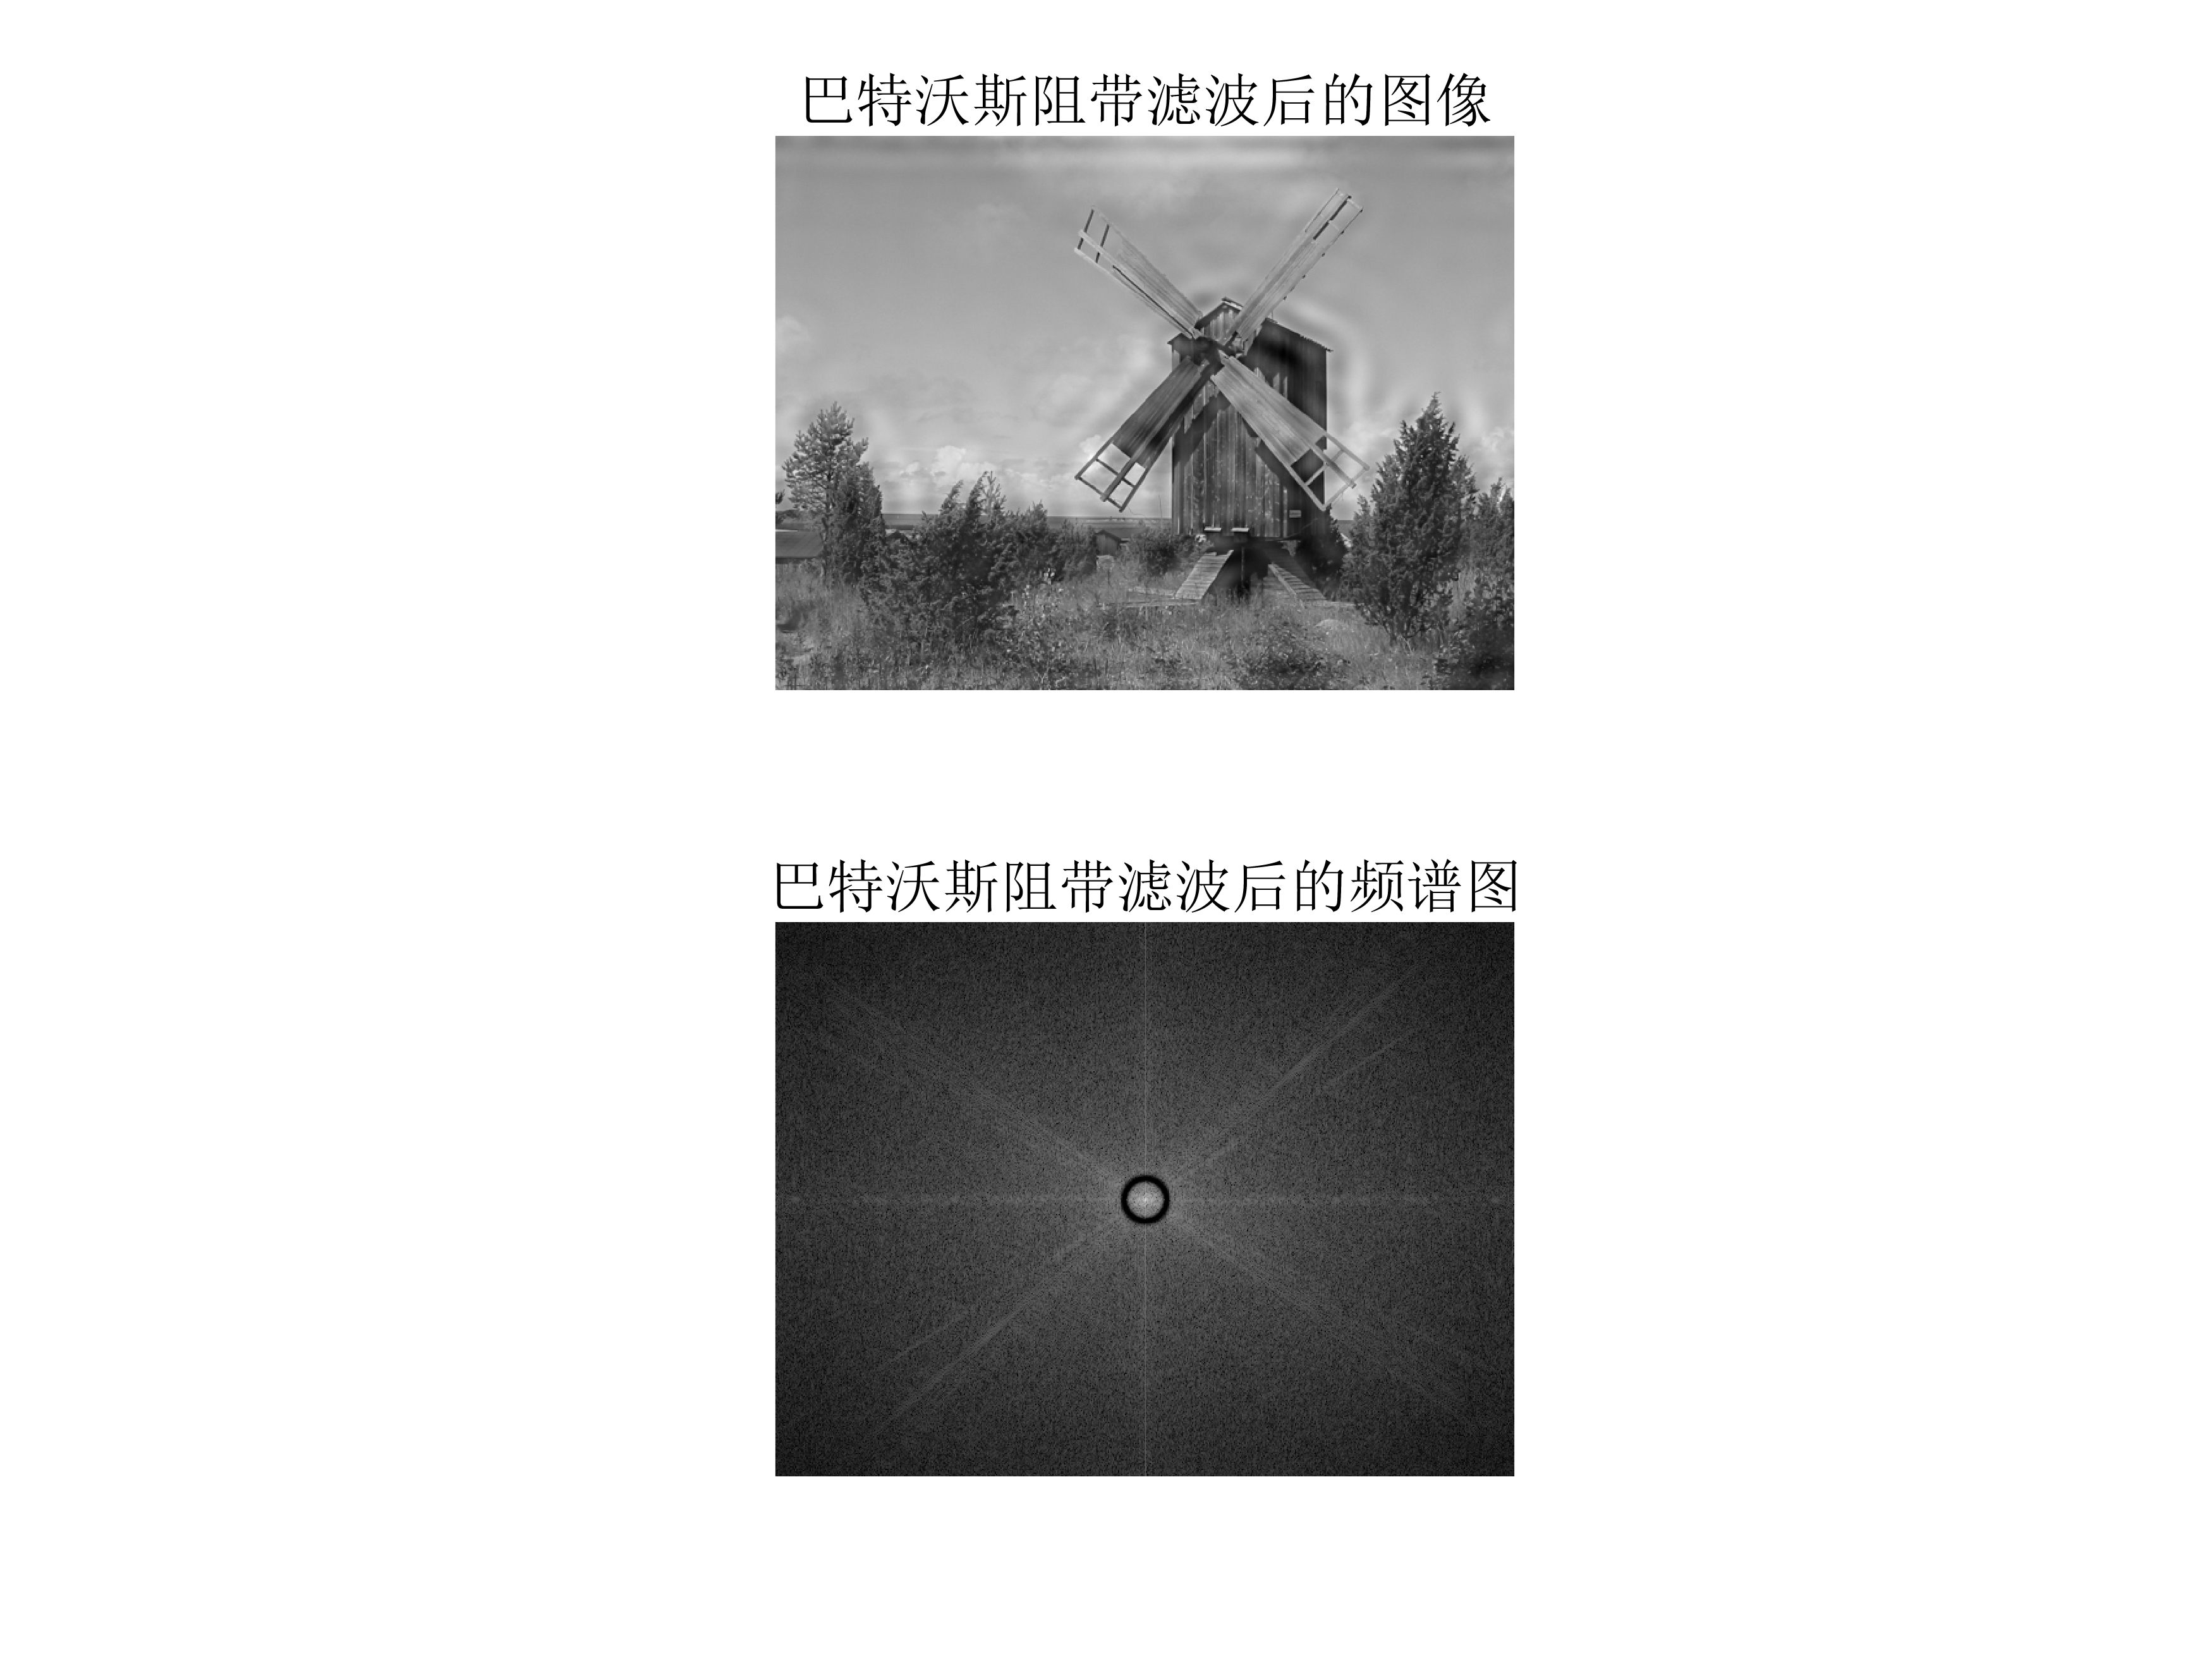
\includegraphics[scale=0.4]{./filtered_img.png}
%                                    %\caption{原图3}
%                                \end{minipage}
%                            }
%                            \subfigure[巴特沃斯带阻滤波后的频谱图]{
%                                \begin{minipage}{0.45\linewidth}
%                                    \centering
%                                    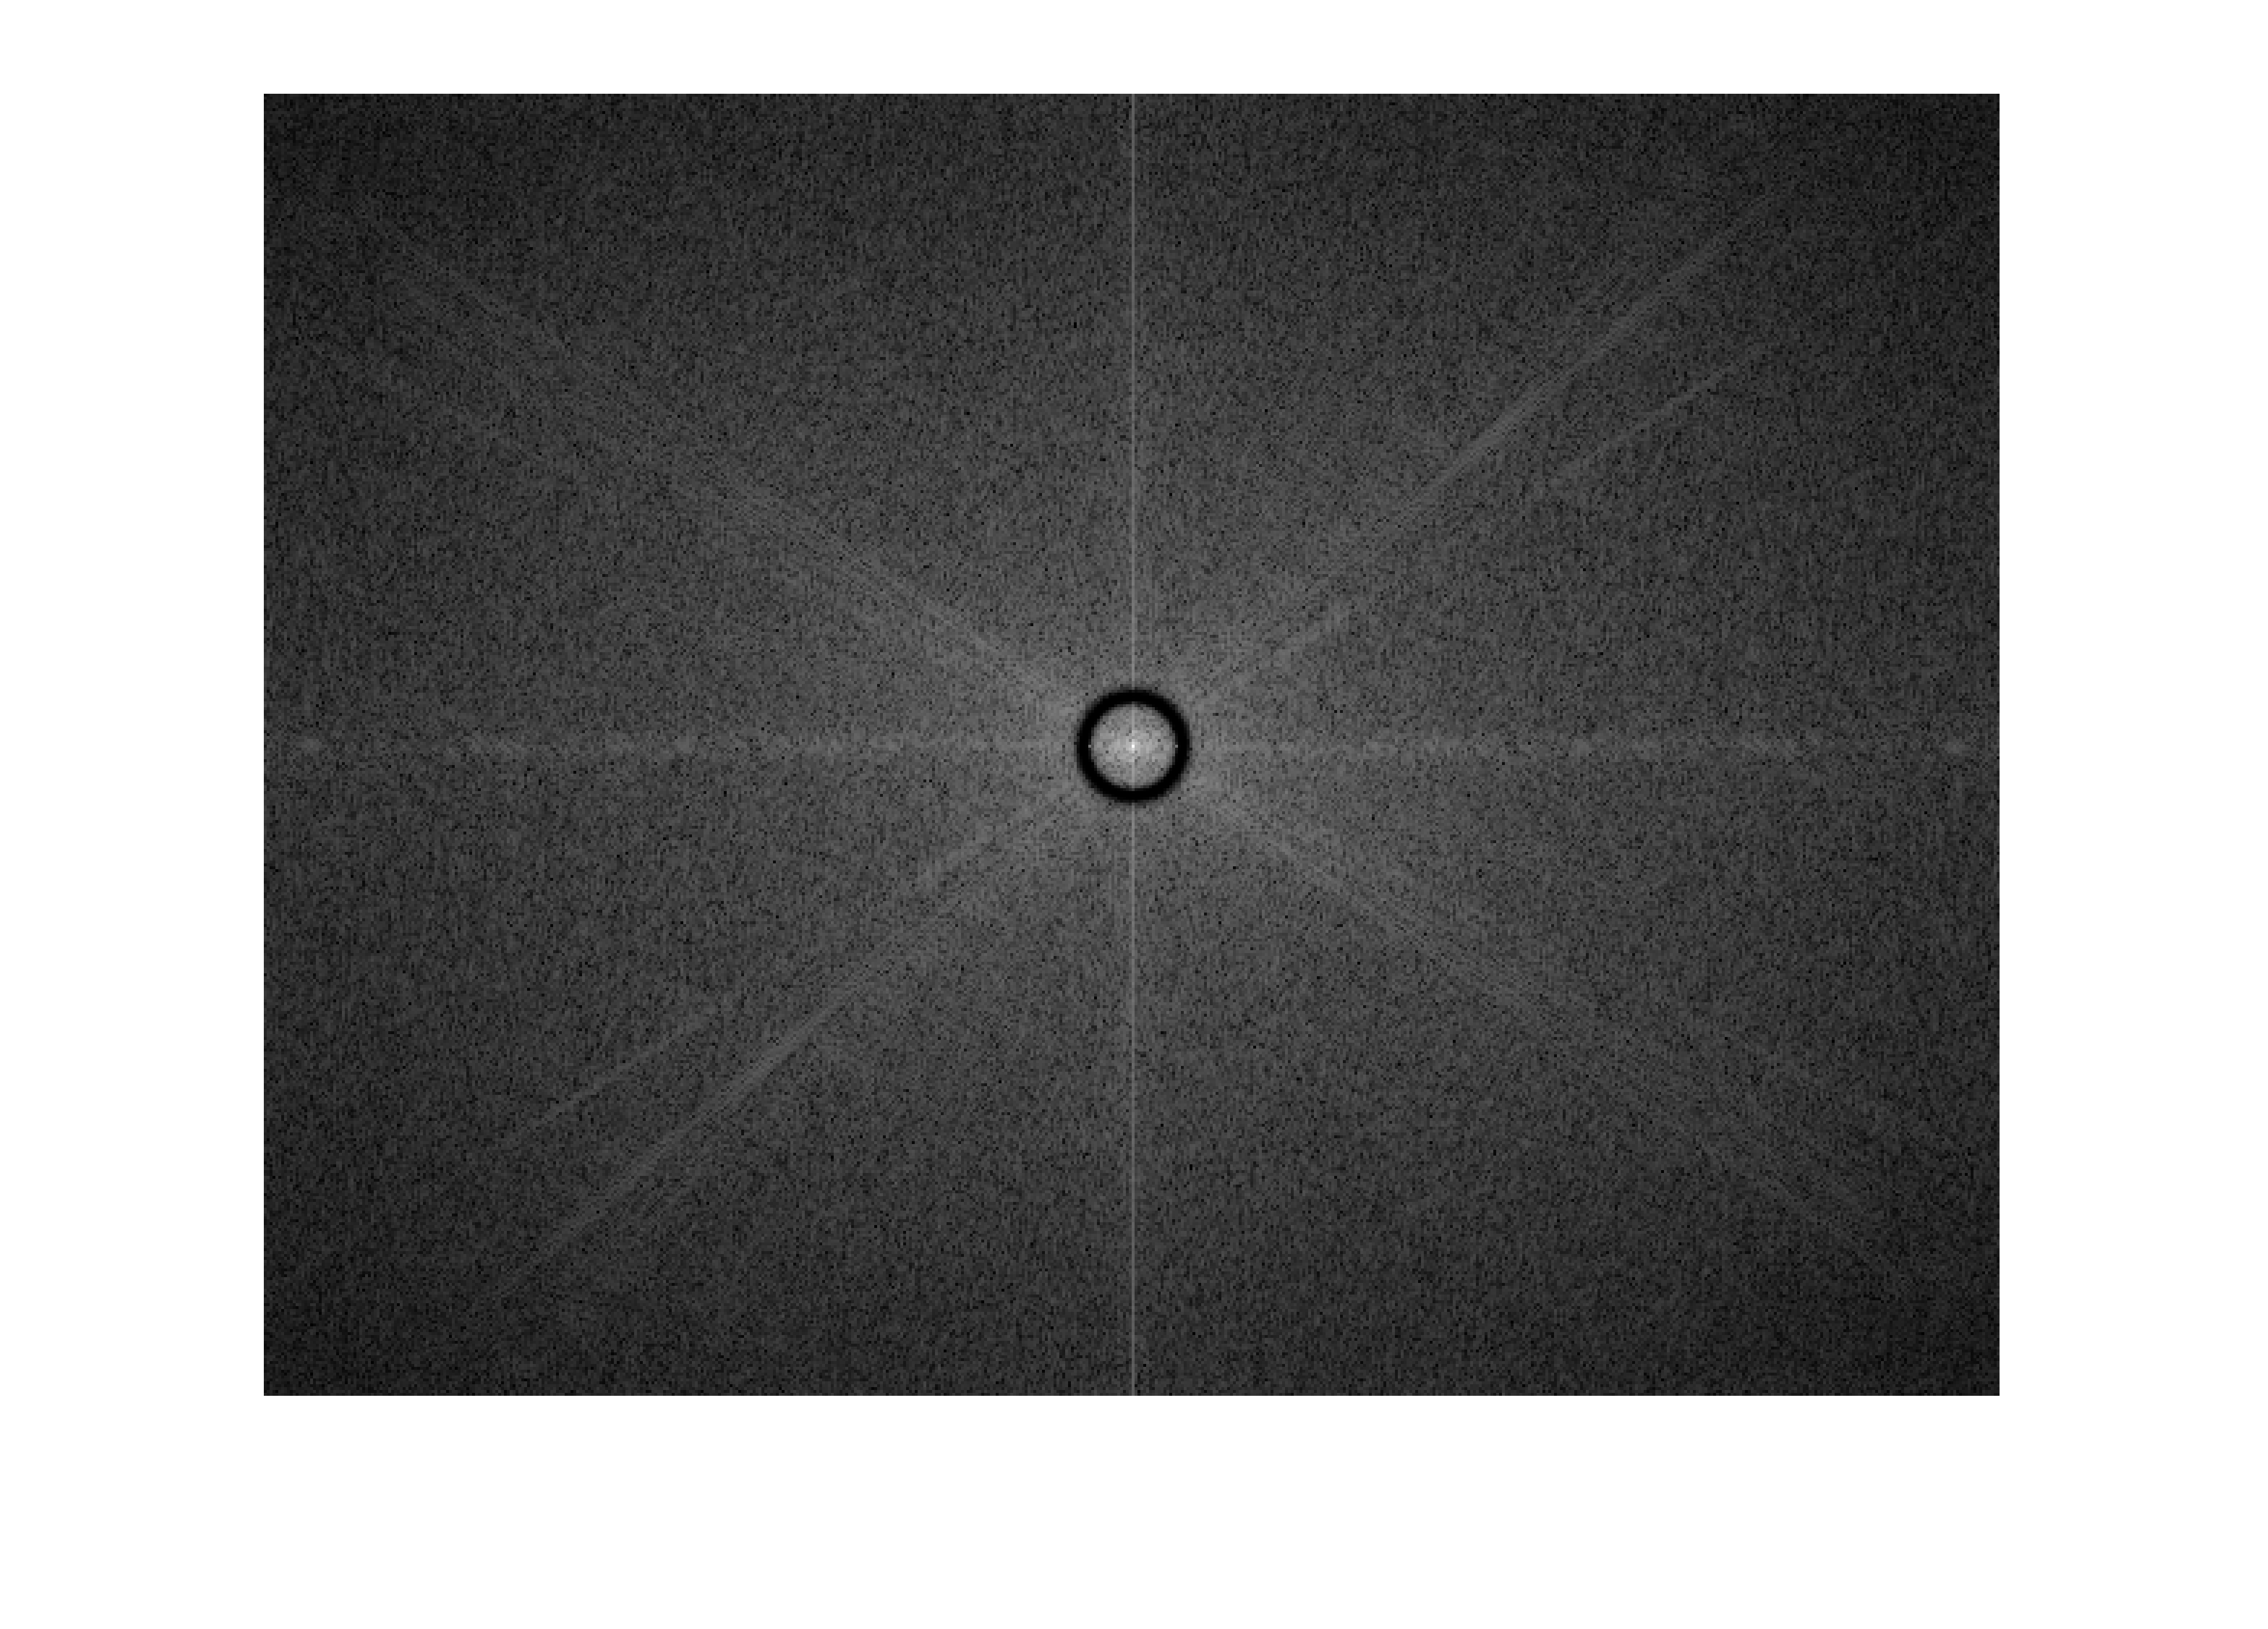
\includegraphics[scale=0.4]{./filtered_spectrum.png}
%                                    %\caption{结果3}
%                                    \label{res4-4}
%                                \end{minipage}
%                            }
%                            
%                            \caption{测试结果}
%                            \label{butterworth}
%                        \end{figure}                        
%                      
%                        \begin{figure}[H]
%                            \centering
%                            \subfigure[高斯带阻滤波后的图像]{
%                                \begin{minipage}{0.45\linewidth}
%                                    \centering
%                                    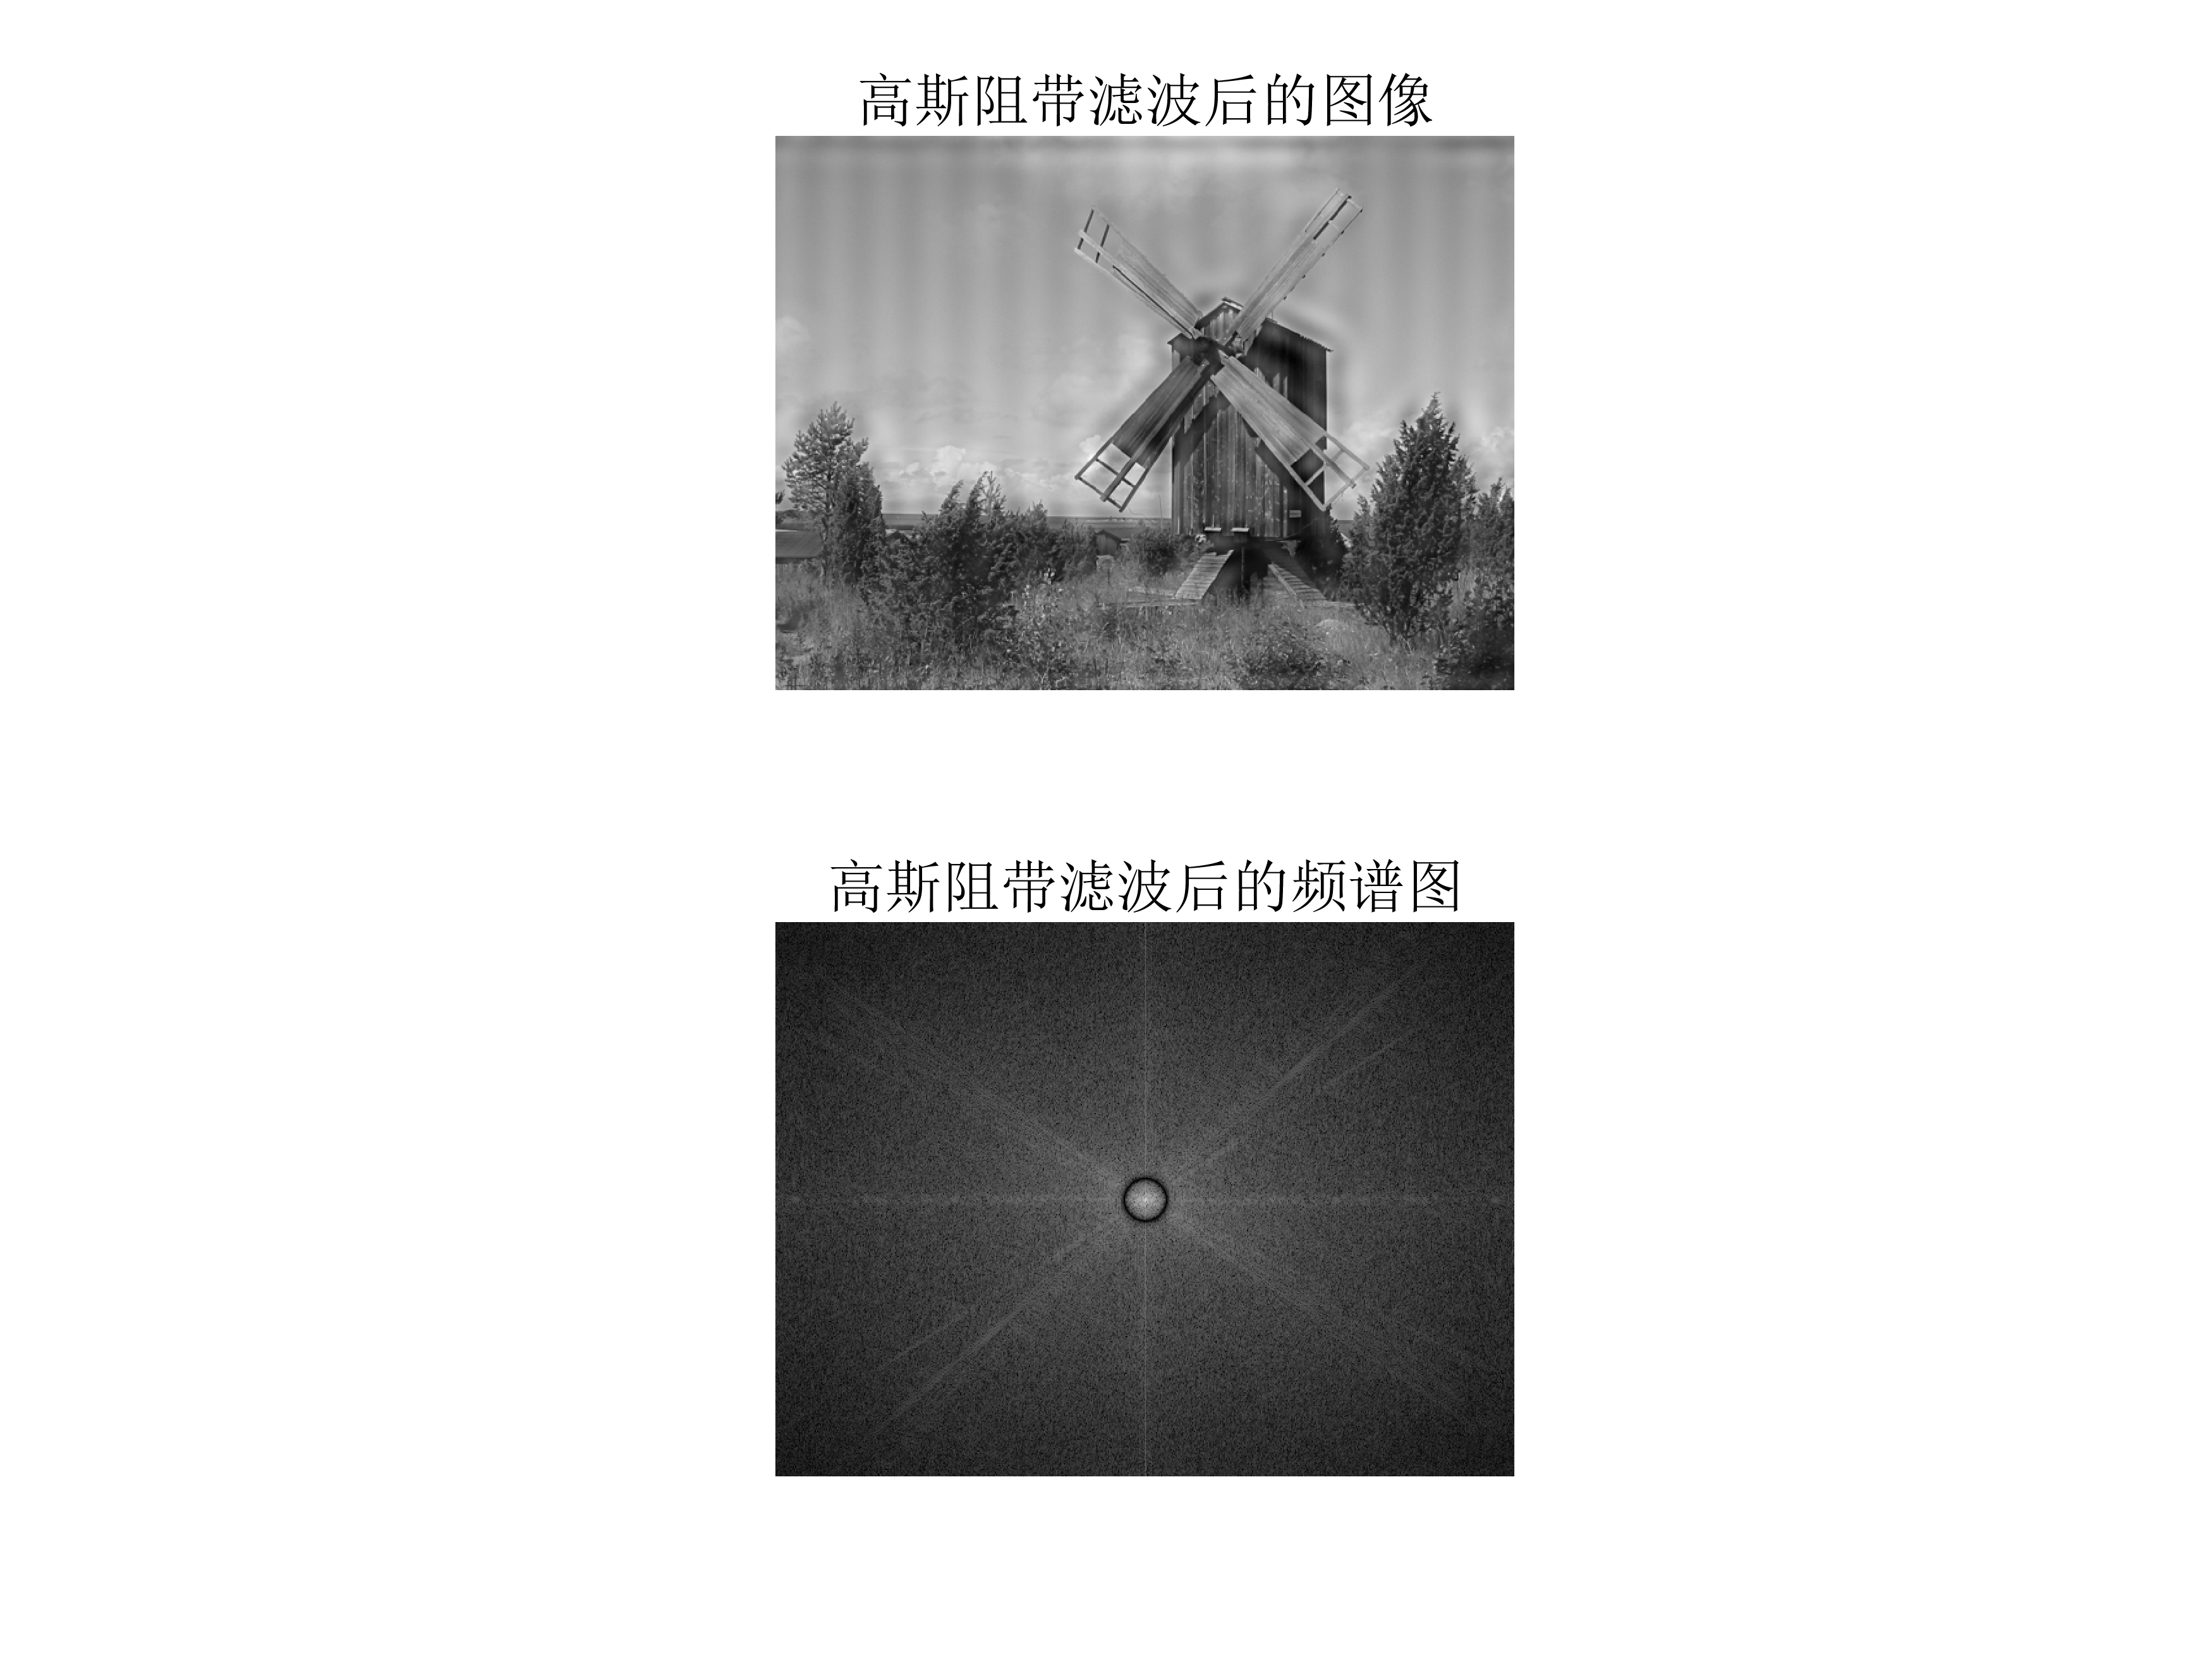
\includegraphics[scale=0.4]{./Gaussian_filtered_img.png}
%                                    %\caption{原图3}
%                                \end{minipage}
%                            }
%                            \subfigure[高斯带阻滤波后的频谱图]{
%                                \begin{minipage}{0.45\linewidth}
%                                    \centering
%                                    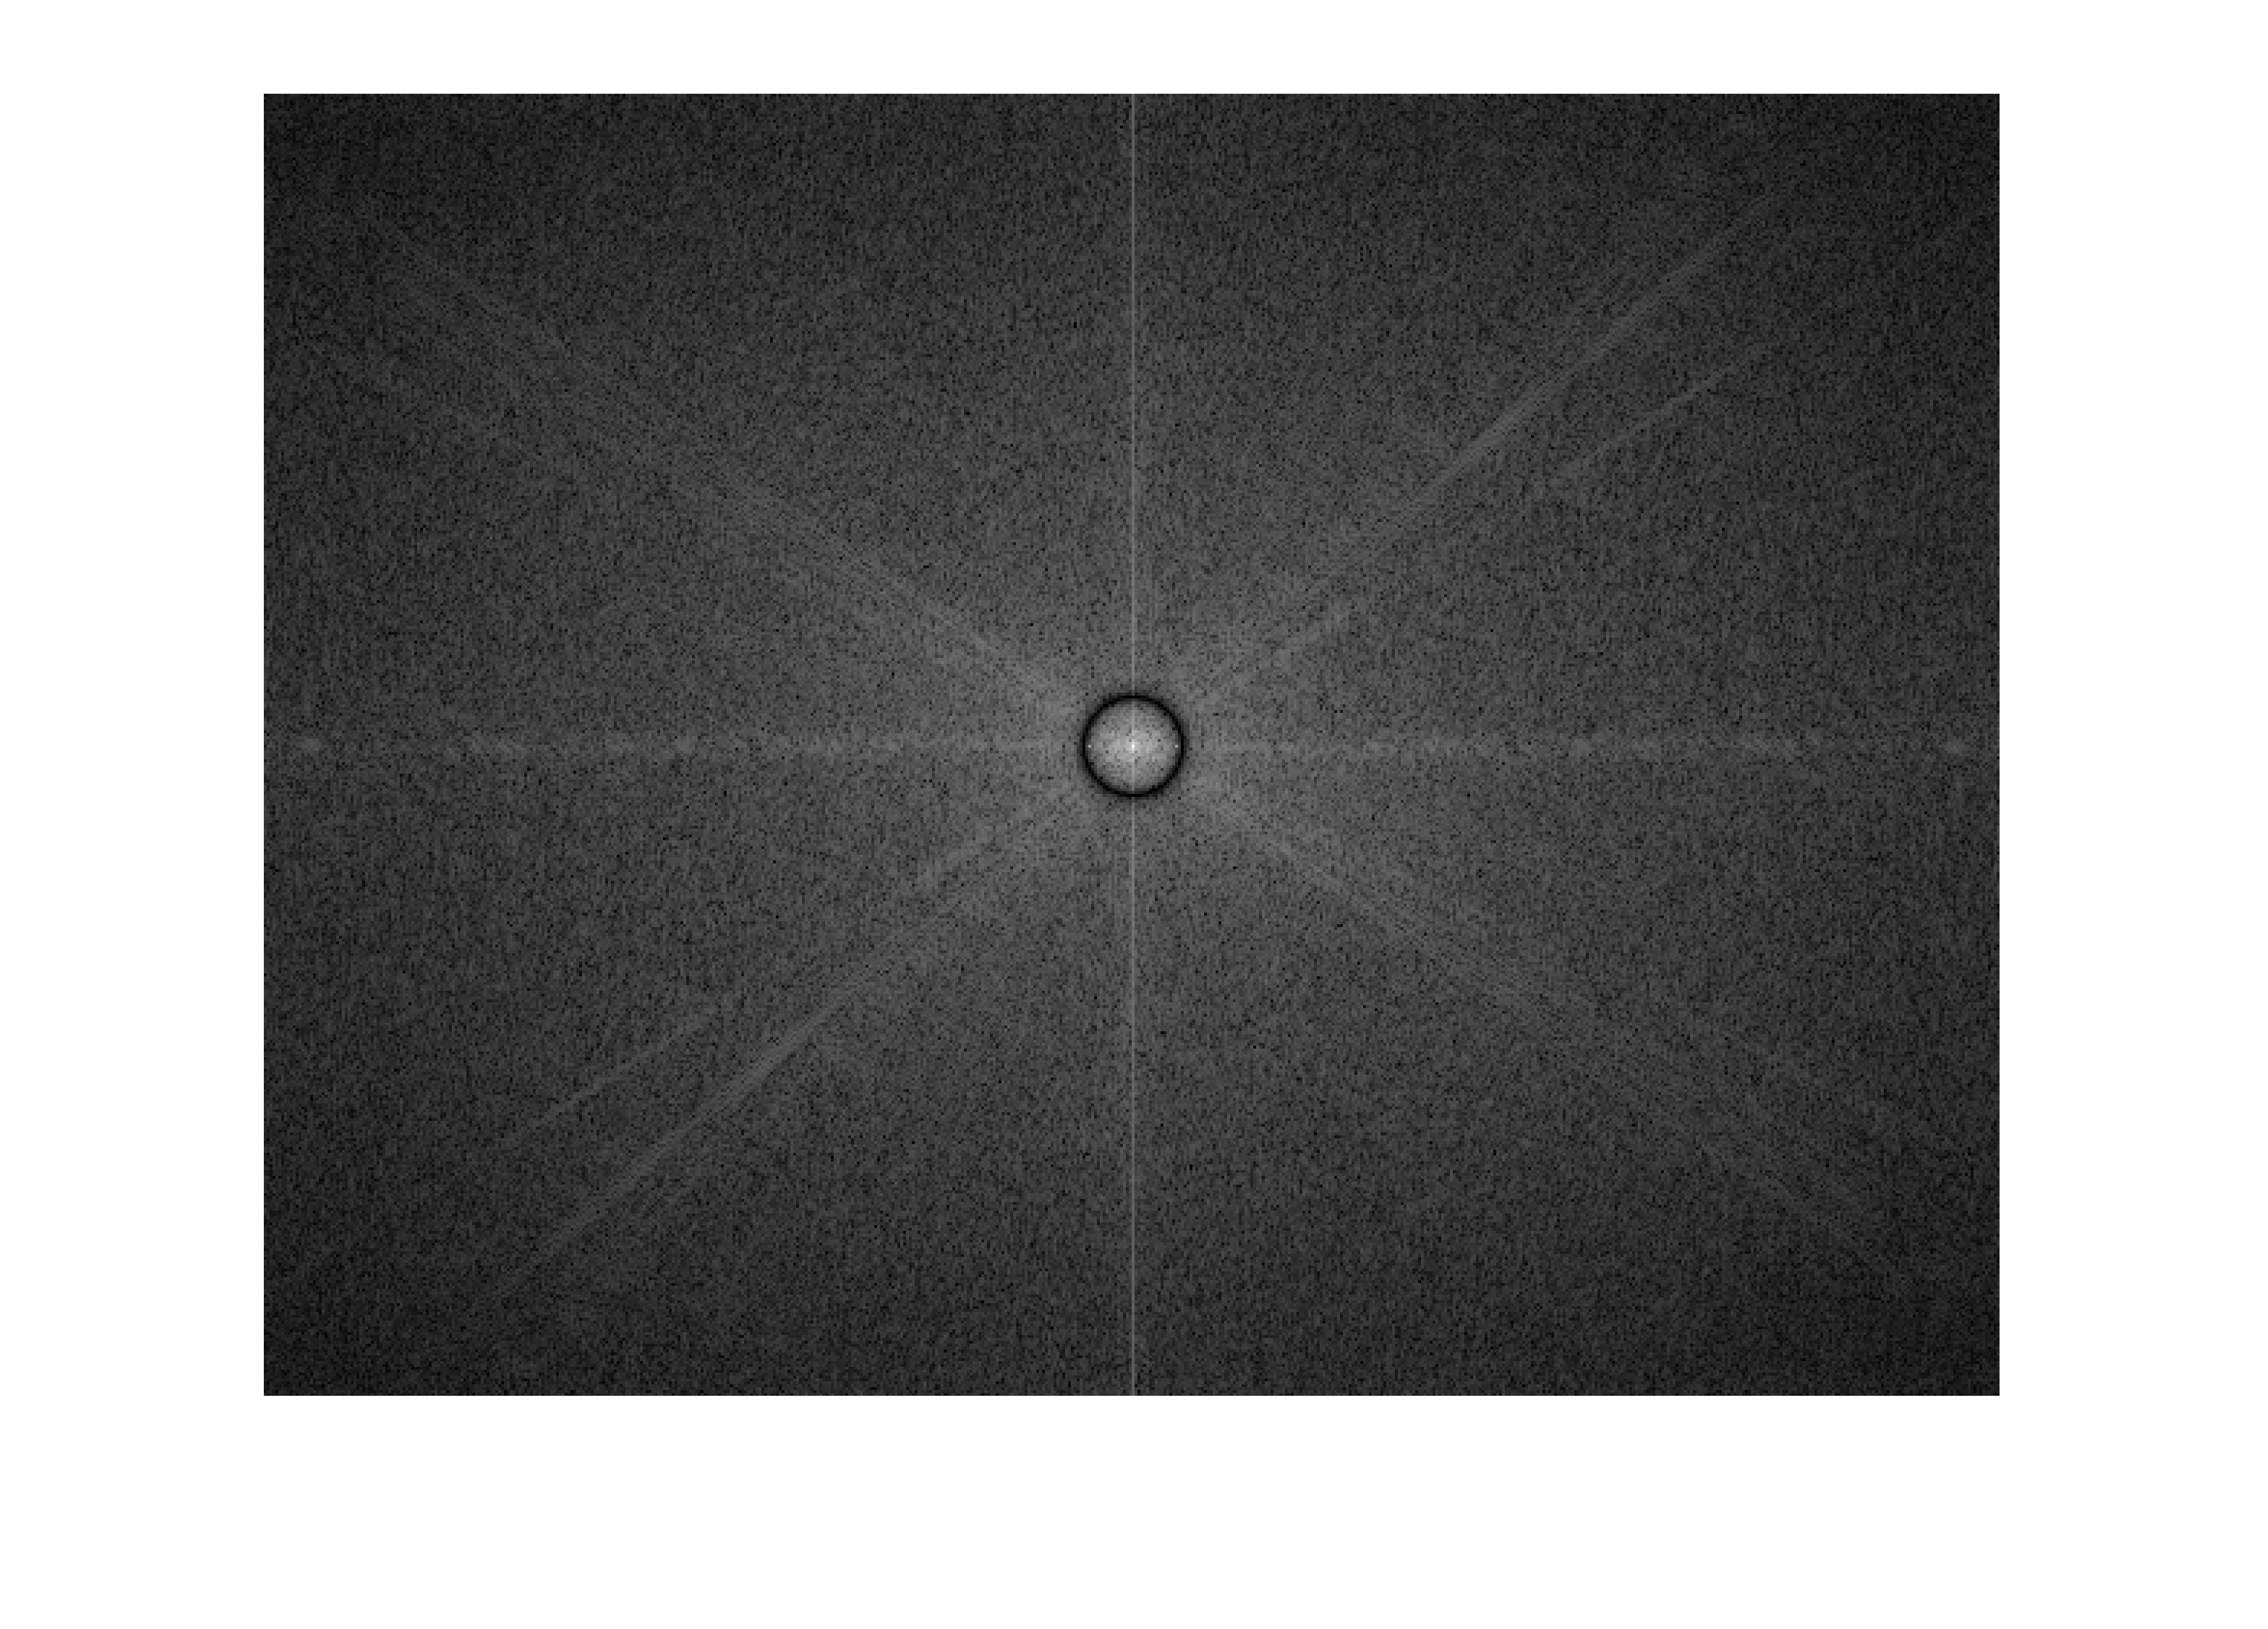
\includegraphics[scale=0.4]{./Gaussian_filtered_spectrum.png}
%                                    %\caption{结果3}
%                                    \label{res4-4}
%                                \end{minipage}
%                            }
%                            
%                            \caption{测试结果}
%                            \label{gaussian}
%                        \end{figure}                              
%                        
    
                            
                                   

	\section{总结}
		
        \indent 本次实验是用$jpeg2000$标准对图像进行压缩,并观察在不同尺度和步长下压缩率大小和解压缩后的图像效果。从图\ref{n=1, Q=[8,8.5]}到图\ref{n=8, Q=[8,8.5]}可以看出,尺度越大,压缩率越大,同时解压缩后的图像质量也越差;从图\ref{n=5, Q=[8,8.5]}以及图\ref{n=5, Q=[8,7]}到图\ref{n=5, Q=[10,8.5]}可以看出,减小步长向量的第二个元素的值会显著提高压缩率,增大则会减小压缩率;而改变第一个元素的值则对结果的影响很小。
        
        
        
%			\begin{figure}[H]
%				\centering 
%				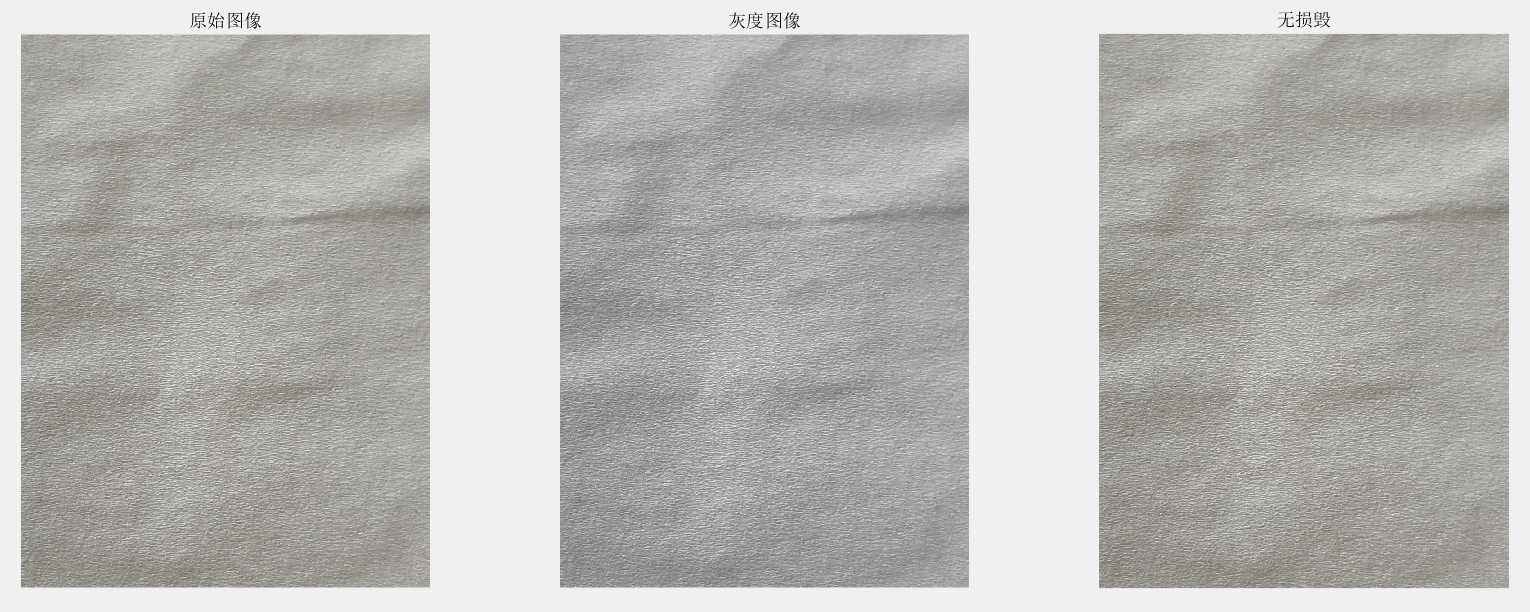
\includegraphics[scale=0.4]{res4.png} 
%				\caption{结果4} 
%				\label{res4}
%			\end{figure}
		

		
%			\begin{figure}[H]
%				\centering 
%				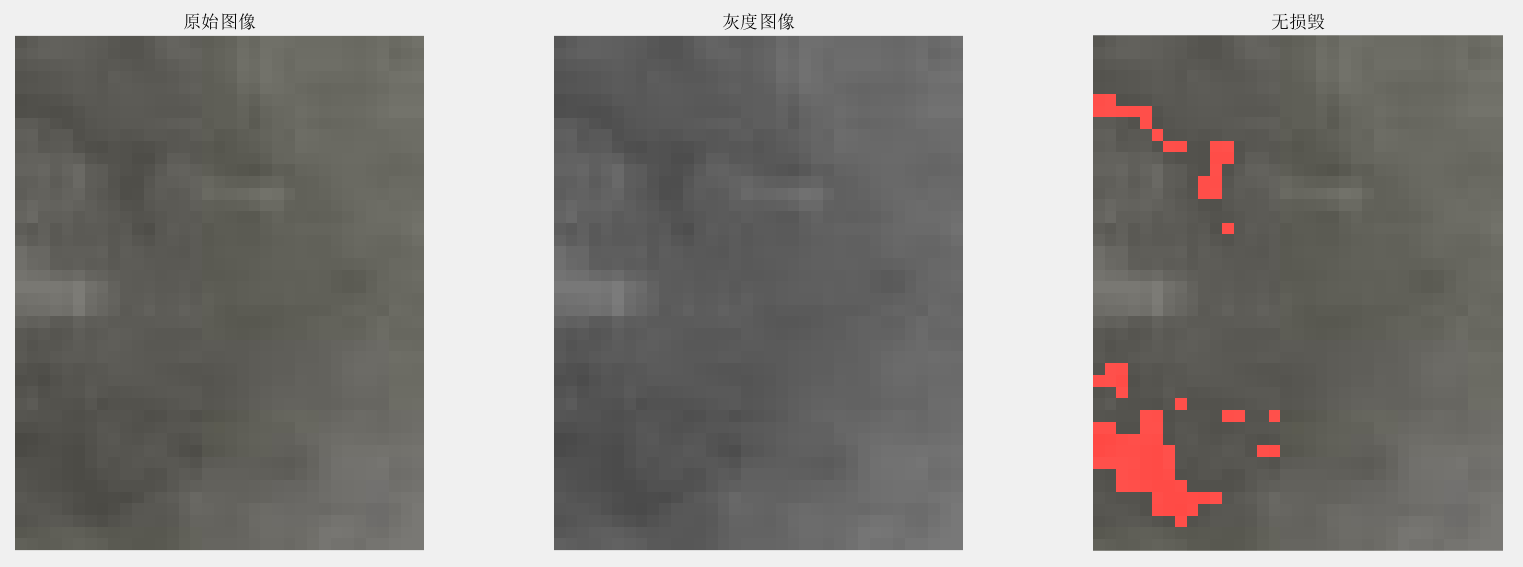
\includegraphics[scale=0.4]{res6.png} 
%				\caption{结果6(截取自结果5的阴影部分)} 
%				\label{res6}
%			\end{figure}
	
	
% 中文文献多个作者用中文逗号“,”连接
%\bibliography{ref.bib}
%\bibliographystyle{abbrv}
\bibliography{ref.bib}


\end{document}